\حصہ{ایک سے زائد بلا منصوبہ متغیرات کی تقسیمیں}\شناخت{حصہ_شماریات_ایک_سے_زائد_متغیرات_تقسیمیں}
اگر ایک بلا منصوبہ تجربہ میں ہم ایک مقدار کا مشاہدہ کریں تب ہمیں اس تجربہ کے ساتھ واحد ایک بلا منصوبہ متغیر، مثلاً \عددی{X}، وابستہ کرنا ہو گا۔حصہ \حوالہ{حصہ_شماریات_بلا_منصوبہ_متغیرات} سے ہم جانتے ہیں کہ اس کا مطابقتی تفاعل تقسیم \عددی{F(x)=P(X\le x)} اس تقسیم کو مکمل طور پر تعین کرتا ہے، چونکہ ہر وقفہ \عددی{a<X\le b} کے لئے درج ذیل ہو گا۔
\begin{align*}
P(a<X\le b)=F(b)-F(a)
\end{align*}

اگر ایک بلا منصوبہ تجربہ میں ہم دو مقدار کا مشاہدہ کریں تب ہمیں اس تجربہ کے ساتھ دو بلا منصوبہ متغیرات، مثلاً \عددی{X} اور \عددی{Y}، وابستہ کرنا ہو گا۔مثال کے طور پر فولاد کی راک ویل سختی کو  \عددی{X}  اور اس میں کاربن کی مقدار کو \عددی{Y} ظاہر کر سکتے ہیں۔ہر ایک تجربہ اعداد کی جوڑی \عددی{X=x}، \عددی{Y=y} دے گی جس کو مختصراً \عددی{(x,y)} لکھا اور \عددی{XY} مستوی پر بطور نقطہ دکھایا جا سکتا ہے۔ہم اب ایک مستطیل \عددی{a_1<X\le b_1}، \عددی{a_2<Y\le b_2} پر غور کرتے ہیں (شکل \حوالہ{شکل_شماریات_دو_بعدی_تقسیم})۔اگر ایسے ہر ایک مستطیل کے لئے  ہمیں مطابقتی احتمال
\begin{align*}
P(a_1<X\le b_1,\,\, a_2<Y\le b_2)
\end{align*}
معلوم ہو تب ہم کہتے ہیں کہ \اصطلاح{دو بعدی بلا منصوبہ متغیر}\فرہنگ{بلا منصوبہ!دو بعدی متغیر}\حاشیہب{two-dimensional random variable}\فرہنگ{random!two-dimensional variable} \عددی{(X,Y)} یا بلا منصوبہ متغیرات \عددی{X} اور \عددی{Y} کا \اصطلاح{دو بعدی تفاعل احتمال}\فرہنگ{احتمال!دو بعدی تفاعل}\حاشیہب{two-dimensional probability distribution}\فرہنگ{probability!two-dimensional function} ہمیں معلوم ہے۔تفاعل
\begin{align}\label{مساوات_شماریات_ایک_سے_زائد_الف}
F(x,y)=P(X\le x,Y\le y)
\end{align}
کو اس تقسیم یا \عددی{(X,Y)} کا \اصطلاح{تقسیمی تفاعل}\فرہنگ{تقسیمی!تفاعل}\حاشیہب{distribution function}\فرہنگ{distribution!function} کہتے ہیں۔چونکہ (سوال \حوالہ{سوال_شماریات_ایک_سے_زائد_ثبوت_ب})
\begin{gather}
\begin{aligned}\label{مساوات_شماریات_ایک_سے_زائد_ب}
P(a_1&<X\le b_1,a_2<Y\le b_2)\\
&=F(b_1,b_2)-F(a_1,b_2)-F(b_1,a_2)+F(a_1,a_2)
\end{aligned}
\end{gather}
لکھا جا سکتا ہے لہٰذا مساوات \حوالہ{مساوات_شماریات_ایک_سے_زائد_الف} تقسیم کو یکتا طور پر تعین کرتا ہے۔
\begin{figure}
\centering
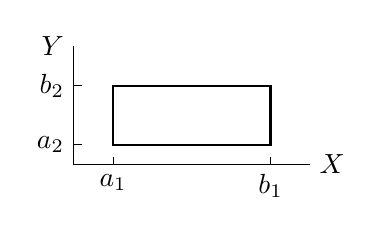
\begin{tikzpicture}
\draw(0,1.5)node[left]{$Y$}--(0,0)--(3,0)node[right]{$X$};
\draw[thick](0.5,0.25) rectangle (2.5,1);
\draw(0.5,0)node[below]{$a_1$}--++(0,0.1);
\draw(2.5,0)node[below]{$b_1$}--++(0,0.1);
\draw(0,0.25)node[left]{$a_2$}--++(0.1,0);
\draw(0,1)node[left]{$b_2$}--++(0.1,0);
\end{tikzpicture}
\caption{دو بعدی تقسیم کا تصور}
\label{شکل_شماریات_دو_بعدی_تقسیم}
\end{figure}

%==================
\جزوحصہء{غیر مسلسل دو بعدی تقسیمیں}
اگر \عددی{(X,Y)} درج ذیل خواص رکھتا ہو تب متغیر \عددی{(X,Y)} اور اس کا مطابقتی تقسیم \اصطلاح{غیر مسلسل}\فرہنگ{غیر مسلسل!تقسیم}\فرہنگ{غیر مسلسل!متغیر}\فرہنگ{discrete!variable}\فرہنگ{discrete!distribution} کہلائے گا۔

\عددی{X,Y} متناہی تعداد یا قابل شمار لامتناہی تعداد کی جوڑی قیمتیں \عددی{(x,y)} اختیار کر سکتا ہے جن کے مطابقتی احتمال مثبت ہوں گے۔ہر ایسا دائرہ کار جس میں ایسی کوئی جوڑی نہ پائی جاتی ہو کا احتمال \عددی{0} ہو گا\حاشیہد{دھیان رہے کہ پہلی خاصیت سے یہ نہیں کہا جا سکتا ہے}۔ 

فرض کریں کہ \عددی{x_i,y_j} ایسی کوئی  جوڑی ہے اور \عددی{P(X=x_i,Y=y_j)=p_{ij}} ہے(جہاں ہم فرض کرتے ہیں کہ \عددی{p_{ij}} کسی مخصوص \عددی{i,j} کی جوڑیوں  کے لئے صفر بھی ہو سکتا ہے)۔ تفاعل
\begin{align}
f(x,y)=
\begin{cases}
p_{ij}& x=x_i,y=y_j\\
0&\text{ورنہ}
\end{cases}
\end{align}
کو \عددی{(X,Y)} کا \اصطلاح{تفاعل احتمال} کہتے ہیں؛ یہاں غیر تابع طور پر \عددی{i=1,2,\cdots} اور \عددی{j=1,2,\cdots} ہیں۔مساوات \حوالہ{مساوات_شماریات_غیر_مسلسل_متغیر_ج} کا مماثل 
\begin{align}
F(x,y)=\sum_{x_i\le x}\sum_{y_j\le y}f(x_i,y_j)
\end{align}
ہے اور مساوات \حوالہ{مساوات_شماریات_غیر_مسلسل_متغیر_پ} کی جگہ درج ذیل شرط ہو گا۔
\begin{align}
\sum_{i}\sum_{j}f(x_i,y_j)=1
\end{align}

مثال کے طور پر اگر ہم ایک روپیہ اور پانچ روپیہ کے سکے اچھال کر 
\begin{align*}
X&=\text{\RL{ایک روپیہ کی خط کی تعداد}}\\
Y&=\text{\RL{پانچ روپیہ کی خط کی تعداد}}
\end{align*}
پر غور کریں تب \عددی{X} اور \عددی{Y} کی قیمت\عددی{0} یا \عددی{1} ہو سکتی ہے اور تفاعل احتمال
\begin{align*}
\text{\RL{ہو گا۔}}\,\, f(x,y)=0\,\,\text{\RL{ورنہ (ان کے علاوہ)}}\,\,f(0,0)=f(1,0)=f(0,1)=f(1,1)=\frac{1}{4}
\end{align*}

%======================
\جزوحصہء{استمراری دو بعدی تقسیمیں}
\عددی{(X,Y)} اور اس کا تقسیم اس صورت استمراری کہلاتے ہیں جب  مطابقتی تفاعل تقسیم کو دوہرا تکمل
\begin{align}
F(x,y)=\int_{-\infty}^{y}\int_{-\infty}^{x}f(x^*,y^*)\dif x^*\dif y^*
\end{align}
کی صورت میں لکھنا ممکن ہو جہاں \عددی{f(x,y)} معین، غیر منفی اور پورے مستوی میں محدود ہے ماسوائے متناہی تعداد کے استمراری قابل تفرق منحنیات پر۔ \عددی{f(x,y)} کو تقسیم کی \اصطلاح{کثافت احتمال} کہتے ہیں۔یوں درج ذیل ہو گا۔
\begin{align}
P(a_1<X\le b_1, a_2<Y\le b_2)=\int_{a_2}^{b_2}\int_{a_1}^{b_1}f(x,y)\dif x\dif y
\end{align}

مثال کے طور پر  (شکل \حوالہ{شکل_شماریات_یکساں_تقسیم_الف})
\begin{align}\label{مساوات_شماریات_یکساں_متعدد_متغیرات_کثافت}
f(x,y)=0\,\text{ورنہ}\,f(x,y)=\frac{1}{k}\,\text{میں ہو تب}\,R\,\text{\RL{مستطیل}} \,(x,y)\,\text{جب}
\end{align}
مستطیل \عددی{R} میں یکساں تقسیم کو ظاہر کرتا ہے؛ یہاں \عددی{k} مستطیل کا رقبہ یعنی \عددی{k=(\beta_1-\alpha_1)(\beta_2-\alpha_2)} ہے۔اس تقسیم کو شکل \حوالہ{شکل_شماریات_یکساں_تقسیم_ب} میں دکھایا گیا ہے۔
\begin{figure}
\centering
\begin{minipage}{0.45\textwidth}
\centering
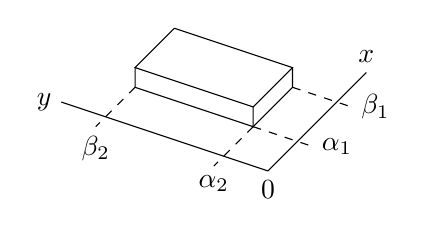
\begin{tikzpicture}[x={(-0.5cm,-0.5cm)},y={(0.75cm,-0.25cm)},z={(0,1cm)}]
\draw(0,0,0.25)--++(1,0,0)--++(0,2,0)--++(-1,0,0)--++(0,-2,0);
\draw(1,0,0.25)--++(0,0,-0.25)--++(0,2,0)--++(0,0,0.25);
\draw(1,2,0)--++(-1,0,0)--++(0,0,0.25);
\draw[dashed] (1,0,0)--++(1,0,0)node[below]{$\beta_2$};
\draw[dashed] (1,2,0)--++(1,0,0)node[below]{$\alpha_2$};
\draw[dashed](0,2,0)--++(0,1,0)node[right]{$\beta_1$};
\draw[dashed](1,2,0)--++(0,1,0)node[right]{$\alpha_1$};
\draw (1.75,2.75)node[below]{$0$}--++(-2.5,0,0)node[above]{$x$};
\draw (1.75,2.75)--++(0,-3.5,0)node[left]{$y$};
\end{tikzpicture}
\caption{یکساں تقسیم (مساوات \حوالہ{مساوات_شماریات_یکساں_متعدد_متغیرات_کثافت}) کا تفاعل احتمال کثافت}
\label{شکل_شماریات_یکساں_تقسیم_الف}
\end{minipage}\hfill
\begin{minipage}{0.45\textwidth}
\centering
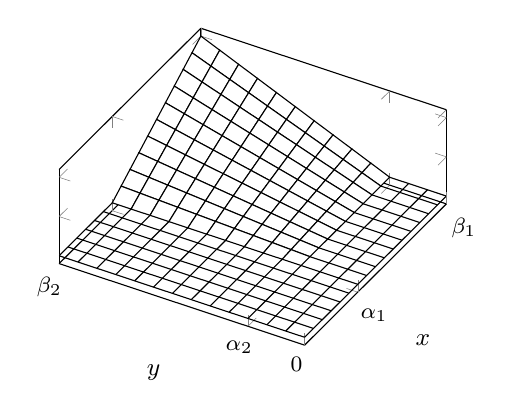
\begin{tikzpicture}
\begin{axis}[small, view={-60}{60},xtick={0.6,1.6},ytick={0,0.6,2.6},xticklabels={$\alpha_1$,$\beta_1$},yticklabels={$0$,$\alpha_2$,$\beta_2$},zticklabels={\empty},xlabel={$x$},ylabel={$y$}]
\addplot3[samples=11,samples y=11,surf,color=white,faceted color=black,domain=0.6:1.6,y domain=0.6:2.6]{(x-0.6)*(y-0.6)};
%the following manually matches the grid lines
\foreach \kk in {0.6,0.8,...,2.6}{
\addplot3 [domain=0:0.6, samples y=1, black,smooth] (x,\kk,0);}
\foreach \kk in {0.6,0.7,...,1.6}{
\addplot3 [domain=0:0.6, samples y=1, black,smooth] (\kk,x,0);}
\foreach \kk in {0,0.2,...,0.58}{
\addplot3 [domain=0:1.6, samples y=1, black,smooth] (x,\kk,0);}
\foreach \kk in {0,0.1,...,0.59}{
\addplot3 [domain=0:2.6, samples y=1, black,smooth] (\kk,x,0);}
\end{axis}
\end{tikzpicture}
\caption{یکساں تقسیم (مساوات \حوالہ{مساوات_شماریات_یکساں_متعدد_متغیرات_کثافت}) کا تفاعل تقسیم}
\label{شکل_شماریات_یکساں_تقسیم_ب}
\end{minipage}%
\end{figure}

%=================
\جزوحصہء{دو بعدی غیر مسلسل تقسیم کے حاشیہ تقسیمیں}
فرض کریں کہ بلا منصوبہ غیر مسلسل متغیر \عددی{(X,Y)} کا تفاعل احتمال \عددی{f(x,y)} ہے۔اگر \عددی{X=x} ہو، جبکہ \عددی{Y} جس میں ہمیں دلچسپی نہیں ہے کوئی بھی قیمت اختیار کر سکتا ہو، تب تفاعل احتمال \عددی{P(X=x,Y \text{اختیاری})} کو \عددی{f_1(x)} لکھا جا سکتا ہے جو \عددی{x} کا تابع تفاعل ہے۔یوں 
\begin{align}\label{مساوات_شماریات_حاشیہ_الف}
f_1(x)=P(X=x,Y\,\text{اختیاری})=\sum_y f(x,y)
\end{align} 
لکھا جا سکتا ہے جہاں اس \عددی{x} کے لئے ہم \عددی{f(x,y)} کی  تمام غیر صفر قیمتوں کا مجموعہ لیا گیا ہے۔ظاہر ہے کہ \عددی{f_1(x)} ایک بلا منصوبہ متغیر تقسیمی احتمال کا تفاعل احتمال ہے۔اس تقسیم کو دیے گئے دو بعدی تقسیم کے لحاظ ہے \عددی{X} کا \اصطلاح{حاشیہ تقسیم}\فرہنگ{تقسیم!حاشیہ}\حاشیہب{marginal distribution}\فرہنگ{distribution!marginal} کہا جاتا ہے۔اس کا تفاعل تقسیم درج ذیل ہو گا۔
\begin{align}\label{مساوات_شماریات_حاشیہ_ب}
F_1(x)=P(X\le x,Y\, \text{اختیاری})=\sum_{x^*\le x} f_1(x^*)
\end{align}
اسی طرح تفاعل احتمال 
\begin{align}\label{مساوات_شماریات_حاشیہ_پ}
f_2(y)=P(X\,\text{اختیاری}, Y=y)=\sum_x f(x,y))
\end{align}
دیے گیے دو بعدی تقسیم کا \عددی{Y} کے لحاظ سے \اصطلاح{حاشیہ تقسیم} تعین کرتا ہے۔مساوات \حوالہ{مساوات_شماریات_حاشیہ_پ} میں ہم \عددی{y} کے مطابقتی غیر صفر \عددی{f(x,y)} کا مجموعہ لیتے ہیں۔اس تقسیم کا تفاعل تقسیم درج ذیل ہو گا۔
\begin{align}
F_2(y)=P(X\,\text{اختیاری},Y\le y)=\sum_{y^*\le y}f_2(y^*)
\end{align}
ظاہر ہے کہ بلا منصوبہ متغیر \عددی{(X,Y)} کے دونوں حاشیہ تقسیم  غیر مسلسل ہیں۔

جدول \حوالہ{جدول_شماریات_تاش_ملکہ_بادشاہ} میں ان کی مثال دی گئی ہے جہاں تاش کے پتوں سے تین پتے نکال کر واپس رکھے جاتے ہیں۔ملکہ کے حصول کو \عددی{X} جبکہ بادشاہ کے حصول کو \عددی{Y} سے ظاہر کیا گیا ہے۔تاش کے کل \عددی{52} پتے ہوتے ہیں جن میں \عددی{4} ملکہ اور \عددی{4} بادشاہ کے پتے ہوتے ہیں۔یوں ایک پتہ نکال کر ملکہ حاصل کرنے کا احتمال \عددی{\tfrac{4}{52}=\tfrac{1}{13}} ہو گا۔یوں ایک پتہ نکال کر ملکہ یا بادشاہ حاصل کرنے کا احتمال \عددی{\tfrac{2}{13}} ہو گا۔اس طرح اس بلا منصوبہ تجربہ کا مطابقتی تفاعل احتمال
\begin{align*}
f(x,y)=\frac{3!}{x!y!(3-x-y)!}\big(\frac{1}{13}\big)^x\big(\frac{2}{13}\big)^y\big(\frac{10}{13}\big)^{3-x-y}\quad \quad (x+y\le 3)
\end{align*}
ہو گا اور ان کے علاوہ \عددی{f(x,y)=0} ہو گا۔جدول \حوالہ{جدول_شماریات_تاش_ملکہ_بادشاہ} میں \عددی{f(x,y)}، \عددی{f_1(x)} اور \عددی{f_2(y)} دیے گئے ہیں۔ 
\begin{table}
\caption{تاش سے ملکہ اور بادشاہ کا حصول}
\label{جدول_شماریات_تاش_ملکہ_بادشاہ}
\centering
\begin{otherlanguage}{english}
\begin{tabular}{C|CCCC||C}
\phantom{xxx}y&\multirow{2}{*}{0}&\multirow{2}{*}{1}&\multirow{2}{*}{2}&\multirow{2}{*}{3}&\multirow{2}{*}{$f_1(x)$}\\
x\phantom{xxx}&&&&&\\
\hline\Tstrut
0&\frac{1000}{2197}&\frac{600}{2197}&\frac{120}{2197}&\frac{8}{2197}&\frac{1728}{2197}\\  \Tstrut \Bstrut \Tstrut \Bstrut
1&\frac{300}{2197}&\frac{120}{2197}&\frac{12}{2197}&0&\frac{432}{2197}\\   \Tstrut \Bstrut   \Tstrut \Bstrut
2&\frac{30}{2197}&\frac{6}{2197}&0&0&\frac{36}{2197}\\   \Tstrut \Bstrut   \Tstrut \Bstrut
3&\frac{1}{2197}&0&0&0&\frac{1}{2197}\\ 
\hline
\hline   \Tstrut \Bstrut
f_2(y)&\frac{1331}{2197}&\frac{726}{2197}&\frac{132}{2197}&\frac{8}{2197}&\\  
\hline
\end{tabular}
\end{otherlanguage}
\end{table}

\جزوحصہء{دو بعدی استمراری تقسیم کے حاشیہ تقسیمیں}
اسی طرح کثافت \عددی{f(x,y)} والے  استمراری متغیر \عددی{X,Y} کے لئے ہم 
\begin{align*}
(X\le x, Y\,\text{اختیاری})\quad \text{یا}\quad (X\le x, -\infty <Y<\infty)
\end{align*}
پر غور کر سکتے ہیں جس کا مطابقتی احتمال
\begin{align*}
F_1(x)=P(X\le x, -\infty<Y<\infty)=\int_{-\infty}^{\infty} \big(\int_{-\infty}^{\infty} f(x^*,y)\dif y\big)\dif x^*
\end{align*}
ہو گا جس میں
\begin{align}
f_1(x)=\int_{-\infty}^{\infty} f(x,y)\dif y
\end{align}
لکھتے ہوئے
\begin{align}
F_1(x)=\int_{-\infty}^{\infty} f_1(x^*)\dif x^*
\end{align}
لکھا جا سکتا ہے۔\عددی{f_1(x)}  اور \عددی{F_1(x)} کو بالترتیب دیے گئے استمراری تقسیم کے لحاظ سے حاشیہ تقسیم \عددی{X} کی  \ترچھا{کثافت} اور \ترچھا{تقسیمی تفاعل} کہتے ہیں۔دیے گئے دو بعدی استمراری تقسیم کے لحاظ سے تفاعل
\begin{align}
f_2(y)=\int_{-\infty}^{\infty} f(x,y)\dif x
\end{align}
کو حاشیہ تقسیم \عددی{Y} کی کثافت اور
\begin{align}
F_2(y)=\int_{-\infty}^{\infty} f_2(y^*)\dif y^*=\int_{-\infty}^{\infty}\int_{-\infty}^{\infty} f(x,y^*)\dif x\dif y^*
\end{align}
کو حاشیہ تقسیم \عددی{Y} کا تقسیمی تفاعل کہتے ہیں۔ہم دیکھتے ہیں کہ استمراری تقسیم کے دونوں حاشیہ تقسیم استمراری ہیں۔

\جزوحصہء{بلا منصوبہ متغیرات کی تابعیت اور غیر تابعیت}
دو بعدی \عددی{(X,Y)} تقسیم جس کا تفاعل تقسیم \عددی{F(x,y)} ہو کے بلا منصوبہ متغیرات \عددی{X} اور \عددی{Y} اس صورت \اصطلاح{غیر تابع}\فرہنگ{تابع!غیر}\فرہنگ{independent} کہلاتے ہیں جب تمام \عددی{(x,y)} کے لئے
\begin{align}
F(x,y)=F_1(x)F_2(y)
\end{align}
ہو ورنہ انہیں \اصطلاح{تابع}\فرہنگ{تابع}\فرہنگ{dependent} کہتے ہیں۔


فرض کریں کہ \عددی{X} اور \عددی{Y} دونوں غیر مسلسل  یا دونوں استمراری ہوں۔تب \عددی{X} اور \عددی{Y} اس صورت غیر تابع ہوں گے جب ان کے مطابقتی تفاعل احتمال یا کثافتیں \عددی{f_1(x)} اور \عددی{f_2(y)} درج ذیل کو مطمئن کرتے ہوں (سوال \حوالہ{سوال_شماریات_غیر_تابعیت_ثبوت})۔
\begin{align}\label{مساوات_شماریات_تابعیت_غیر_تابعیت}
f(x,y)=f_1(x)f_2(y)
\end{align}
مثال کے طور پر جدول \حوالہ{جدول_شماریات_تاش_ملکہ_بادشاہ} میں متغیرات تابع ہیں۔ایک روپیہ اور پانچ روپیہ کے سکے ایک بار  اچھال کر متغیرات
\begin{align*}
X=\text{\RL{ایک روپیہ کے سکے کے خط کی تعداد}},\quad Y=\text{\RL{پانچ روپیہ کے سکے کے خط کی تعداد}}
\end{align*}
\عددی{0} یا \عددی{1} قیمت اختیار کر سکتے ہیں اور یہ متغیرات غیر تابع ہیں۔

تابعیت اور غیر تابعیت کی تصور کو \عددی{n} بعدی تقسیم \عددی{X_1,\cdots,X_n} جس کا تفاعل احتمال
\begin{align*}
F(x_1,\cdots,x_n)=P(X_!\le x_1,\cdots X_n\le x_n)
\end{align*}
ہو کے \عددی{n} بلا منصوبہ متغیرات  تک وسعت دی جا سکتی ہے۔اگر تمام \عددی{x_1,\cdots,x_n} کے لئے
\begin{align}
F(x_1,\cdots,x_n)=F_1(x_1)F_2(x_2)\cdots F_n(n)
\end{align}
ہو جہاں \عددی{X_j} کے حاشیہ تقسیم کا تقسیمی تفاعل \عددی{F_j(x_j)} ہو، یعنی
\begin{align*}
F_j(x_j)=P(X_j\le x_j, X_k\, \text{اختیاری},\, k\ne j)
\end{align*}
تب یہ بلا منصوبہ متغیرات \اصطلاح{غیر تابع} کہلاتے ہیں ورنہ  ان متغیرات کو \اصطلاح{تابع} کہتے ہیں۔

\جزوحصہء{بلا منصوبہ متغیرات کے تفاعل}
فرض کریں کہ بلا منصوبہ متغیر \عددی{(X,Y)} کا تفاعل احتمال یا کثافت \عددی{f(x,y)} اور تقسیمی تفاعل \عددی{F(x,y)} ہیں اور فرض کریں کہ \عددی{g(x,y)} غیر مستقل استمراری تفاعل ہے جو تمام \عددی{(x,y)} پر معین ہے۔تب \عددی{Z=g(X,Y)} بھی بلا منصوبہ متغیر ہو گا۔مثال کے طور پر ہم دو پانسہ پھینکتے ہیں۔پہلے پانسہ عدد \عددی{X} اور دوسرا پانسہ عدد \عددی{Y} دیتا ہے۔ عدد \عددی{Z=X+Y} ان دونوں کا مجموعہ ہے (شکل \حوالہ{شکل_شماریات_تفاعل_تقسیم_ب})۔

اگر \عددی{(X_1,\cdots,X_n) بلا منصوبہ \عددی{n}} بعدی متغیر ہوا ور تمام \عددی{(x_1,\cdots,x_n)} پر  \عددی{g(x_1,\cdots,x_n)} معین غیر مستقل استمراری تفاعل ہو  تب \عددی{Z=g(X_1,\cdots,X_n)} بھی بلا منصوبہ متغیر ہو گا۔

غیر مسلسل بلا منصوبہ متغیر \عددی{(X,Y)} کی صورت میں ان تمام \عددی{f(x,y)} کا مجموعہ لیتے ہوئے جن کے لئے \عددی{g(x,y)} کی قیمت زیر غور \عددی{y} کے برابر ہو،  ہم \عددی{Z=g(X,Y)} کا تفاعل احتمال \عددی{f(z)} حاصل کر سکتے ہیں، یعنی:
\begin{align}
f(z)=P(Z=z)=\underset{g(x,y)=z}{\sum\sum} f(x,y)
\end{align}
\عددی{Z} کا تقسیمی تفاعل
\begin{align}
F(z)=P(Z\le z)=\underset{g(x,y)\le z}{\sum\sum} f(x,y)
\end{align}
ہے جہاں ہم ان \عددی{f(x,y)} کا مجموعہ لیا جائے گا جن کے لئے \عددی{g(x,y)\le z} ہو۔

بلا منصوبہ استمراری متغیر \عددی{(X,Y)} کے لئے اسی طرح
\begin{align}
F(z)=P(Z\le z) =\underset{g(x,y)\le z}{\int\int} f(x,y)\dif x\dif y
\end{align}
ہو گا جہاں ہر \عددی{z} کے لئے ہم \عددی{xy} مستوی میں خطہ \عددی{g(x,y)\le z} پر تکمل حاصل کرتے ہیں۔

\جزوحصہء{\عددی{g(X,Y)} کی حسابی توقع۔مجموعہ  اوسط اور تغیریت}
درج ذیل عدد کو \عددی{g(X,Y)} کی \اصطلاح{حسابی توقع}\فرہنگ{توقع!حسابی}\حاشیہب{mathematical expectation}\فرہنگ{expectation!mathematical} یا مختصراً \اصطلاح{توقع} کہتے ہیں۔
\begin{align}
E(g(X,Y))=
\begin{cases}
\sum\limits_x \sum\limits_y g(x,y)f(x,y)\quad\quad\quad\quad [(X,Y)\,\text{غیر مسلسل}]   \\[2ex]
\int\limits_{-\infty}^{\infty}\int\limits_{-\infty}^{\infty} g(x,y)f(x,y)\dif x\dif y\quad [(X,Y)\, \text{استمراری}]
\end{cases}
\end{align}
یہاں ہم فرض کرتے ہیں کہ دوہرا مجموعہ حتمی مرتکز ہے اور  \عددی{xy} مستوی پر \عددی{\abs{g(x,y)}f(x,y)} کا تکمل موجود ہے۔درج ذیل کلیہ کو سوال \حوالہ{سوال_شماریات_خطی_مجموعہ_کلیہ} کی طرز پر ثابت کیا جا سکتا ہے۔
\begin{align}\label{مساوات_شماریات_خطی_اوسط_عمومی}
E(ag(X,Y)+bh(X,Y))=aE(g(X,Y))+bE(h(X,Y))
\end{align} 
اس کے ایک مخصوص صورت \عددی{E(X+Y)=E(X)+E(Y)} ہے اور الکراجی ماخوذ سے  درج ذیل حاصل ہوتا ہے۔

%========================
\ابتدا{مسئلہ}\شناخت{مسئلہ_شماریات_مجموعہ_اوسط}\quad \موٹا{(مجموعہ اوسط)}\\
بلا منصوبہ متغیرات کے مجموعے کی اوسط (توقع) ان کے انفرادی اوسط کا مجموعہ ہو گا، یعنی:
\begin{align}
E(X_1+X_2,\cdots+X_n)=E(X_1)+E(X_2)+\cdots+E(X_n)
\end{align}
\انتہا{مسئلہ}
%======================

مزید درج ذیل با آسانی حاصل کیا جا سکتا ہے۔

%===============
\ابتدا{مسئلہ}\شناخت{مسئلہ_شماریات_اوسط_حاصل_ضرب}\quad \موٹا{اوسطوں کا حاصل ضرب}\\
\موٹا{غیر تابع} بلا منصوبہ متغیرات کے حاصل ضرب کی اوسط ان کے انفرادی اوسط کے حاصل ضرب کے برابر ہو گا، یعنی:
\begin{align}\label{مساوات_شماریات_حاصل_ضرب_اوسط}
E(X_1X_2\cdots X_n)=E(X_1)E(X_2)\cdots E(X_n)
\end{align}
\انتہا{مسئلہ}
%========================
\ابتدا{ثبوت}\quad
فرض کریں کہ \عددی{X} اور \عددی{Y} بلا منصوبہ متغیرات ہیں (جہاں دونوں غیر مسلسل یا دونوں استمراری ہیں)۔ تب \عددی{E(XY)=E(X)E(Y)} ہو گا۔ غیر مسلسل صورت میں 
\begin{align*}
E(XY)=\sum_x\sum_y xyf(x,y)=\sum_x xf_1(x)\sum_y y f_2(y)=E(X)E(Y)
\end{align*}
لکھا جا سکتا ہے  اور استمراری صورت میں بھی ثبوت اسی طرح کا ہے۔اس نتیجہ کو \عددی{n} غیر تابع متغیرات تک وسعت دینے سے  مساوات \حوالہ{مساوات_شماریات_حاصل_ضرب_اوسط} ثابت ہوتی ہے۔یوں ثبوت مکمل ہوتا  ہے۔
\انتہا{ثبوت}
%===========================
 
ہم اب تغیریت کے مجموعہ پر غور کرتے ہیں۔فرض کریں کہ \عددی{Z=X+Y} ہے اور \عددی{Z} کی اوسط \عددی{\mu} اور تغیریت \عددی{\sigma^{\,2}} ہے۔سوال \حوالہ{سوال_شماریات_تغیریت_دوسرا_کلیہ} سے درج ذیل لکھا جا سکتا ہے۔
\begin{align*}
\sigma^{\,2}=E([Z-\mu]^2)=E(Z^2)-[E(Z)]^2
\end{align*}
مساوات \حوالہ{مساوات_شماریات_خطی_اوسط_عمومی} سے  دائیں ہاتھ پہلے جزو کو
\begin{align*}
E(Z^2)=E(X^2+2XY+Y^2)=E(X^2)+2E(XY)+E(Y^2)
\end{align*}
لکھا جا سکتا ہے جبکہ دائیں ہاتھ دوسرے جزو کو مسئلہ \حوالہ{مسئلہ_شماریات_اوسط_حاصل_ضرب} کی مدد سے
\begin{align*}
[E(Z)]^2=[E(X)+E(Y)]^2=[E(X)]^2+2E(X)E(Y)+[E(Y)]^2
\end{align*}
لکھا جا سکتا ہے۔انہیں \عددی{\sigma^{\,2}} کے کلیہ میں پر کرتے ہوئے درج ذیل حاصل ہوتا ہے۔
\begin{align*}
\sigma^{\,2}&=E(X^2)-[E(X)]^2+E(Y^2)-[E(Y)]^2\\
&\quad +2[E(XY)-E(X)E(Y)]
\end{align*}
سوال \حوالہ{سوال_شماریات_تغیریت_دوسرا_کلیہ} سے ہم دیکھتے ہیں کہ دائیں ہاتھ پہلی لکیر پر دیا گیا تعلق \عددی{X} اور \عددی{Y} کی تغیریت کا مجموعہ ہے  جنہیں ہم  بالترتیب \عددی{\sigma_1^2} اور \عددی{\sigma_2^2} سے ظاہر کرتے ہیں۔دوسری لکیر پر مقدار
\begin{align}
\sigma_{XY}=E(XY)-E(X)E(Y)
\end{align}
کو \عددی{X} اور \عددی{Y} کی \اصطلاح{باہمی تغیریت}\فرہنگ{تغیریت!باہمی}\حاشیہب{covariance}\فرہنگ{covariance} کہتے ہیں۔اس طرح درج ذیل حاصل ہوتا ہے۔
\begin{align}
\sigma^{\,2}=\sigma_1^2+\sigma_2^2+2\sigma_{XY}
\end{align}
اگر \عددی{X} اور \عددی{Y} غیر تابع ہوں تب \عددی{E(XY)=E(X)E(Y)} لہٰذا \عددی{\sigma_{XY}=0}  اور
\begin{align}
\sigma^{\,2}=\sigma_1^2+\sigma_2^2
\end{align}
ہو گا۔دو سے زائد متغیرات تک وسعت دیتے ہوئے درج ذیل حاصل ہو گا۔

%=============================
\ابتدا{مسئلہ}\شناخت{مسئلہ_شماریات_تغیرات_کا_مجموعہ}\quad \موٹا{(تغیرات کا مجموعہ)}\\
\موٹا{غیر تابع} بلا منصوبہ متغیرات کے مجموعہ کی تغیریت ان متغیرات کے انفرادی تغیریت کے مجموعہ کے برابر ہو گا۔
\انتہا{مسئلہ}
%===========================

\حصہء{سوالات}

\ابتدا{سوال}\شناخت{سوال_شماریات_ایک_سے_زائد_ثبوت_ب}\quad
مساوات \حوالہ{مساوات_شماریات_ایک_سے_زائد_ب} کو ثابت کریں۔\\
جواب:\quad
 شکل \حوالہ{شکل_سوال_شماریات_ایک_سے_زائد_ثبوت_ب} میں \عددیء{(X,Y)}  احتمال \عددی{F(b_1,b_2)} کے ساتھ \عددی{A}، \عددی{B}، \عددی{C} یا \عددی{D} سے قیمت اختیار کر سکتا ہے، احتمال \عددی{F(a_1,b_2)} کے ساتھ \عددی{A} یا \عددی{C} سے قیمت اختیار کر سکتا ہے، احتمال \عددی{F(b_1,a_2)} کے ساتھ \عددی{C} یا \عددی{D} سے قیمت اختیار کر سکتا ہے، احتمال \عددی{F(a_1,a_2)} کے ساتھ \عددی{C} سے قیمت اختیار کر سکتا ہے لہٰذا \عددی{B} سے قیمت حاصل کرنے کا احتمال مساوات \حوالہ{مساوات_شماریات_ایک_سے_زائد_ب} کا دایاں ہاتھ دے گا۔ 
\begin{figure}
\centering
\begin{tikzpicture}
\draw(0,0)node[left]{$Y=b_2$}--++(4,0)--++(0,-2.5)node[below]{$X=b_1$};
\draw(0,-1)node[left]{$Y=a_2$}--++(4,0);
\draw(1.75,0)--++(0,-2.5)node[below]{$X=a_1$};
\draw(1,-0.5)node[]{$A$}  (3,-0.5)node[]{$B$} (1,-1.5)node[]{$C$}  (3,-1.5) node[]{$D$};
\end{tikzpicture}
\caption{شکل برائے سوال \حوالہ{سوال_شماریات_ایک_سے_زائد_ثبوت_ب}}
\label{شکل_سوال_شماریات_ایک_سے_زائد_ثبوت_ب}
\end{figure}
\انتہا{سوال}
%=====================
\ابتدا{سوال}\quad
شکل \حوالہ{شکل_شماریات_یکساں_تقسیم_الف} اور شکل \حوالہ{شکل_شماریات_یکساں_تقسیم_ب} میں دیے تقسیم کے حاشیہ تقسیم حاصل کریں۔
\انتہا{سوال}
%======================
\ابتدا{سوال}\quad
فرض کریں کہ \عددی{8\le x \le 12} اور \عددی{0\le y\le 2} میں \عددی{f(x,y)=k} جبکہ باقی جگہوں پر \عددی{f=0}۔ \عددی{k}، \عددی{P(X\le 11, 1\le Y\le 1.5)} اور \عددی{P(9\le X\le 12, Y\le 1)} تلاش کریں۔\\
جواب:\quad
$\tfrac{1}{8}, \tfrac{3}{16},\tfrac{3}{8}$
\انتہا{سوال}
%======================
\ابتدا{سوال}\quad
ایک کاغذ کی اوسط کمیت \عددی{\SI{10}{\gram}} اور معیاری انحراف \عددی{\SI{0.05}{\gram}} ہے۔ ایسی \عددی{\num{10000}} کاغذوں کی ڈھیر کی اوسط کمیت اور تغیریت کیا ہو گی؟  
\انتہا{سوال}
%=========================
\ابتدا{سوال}\quad
فرض کریں کہ \عددی{x>0}، \عددی{y>0} اور \عددی{x+y<3} میں \عددی{f(x,y)=k} جبکہ باقی جگہوں پر \عددی{f=0} ہے۔\عددی{k} تلاش کریں۔ \عددی{f(x,y)} ترسیم کریں۔ \عددی{P(X+Y\le 1)} اور \عددی{P(Y>X)}  تلاش کریں۔\\
جواب:\quad
$\tfrac{2}{9}, \tfrac{1}{9},\tfrac{1}{2}$
\انتہا{سوال}
%========================
\ابتدا{سوال}\quad 
ایک خالی ڈبے کی اوسط \عددی{\SI{2}{\kilo\gram}} اور معیاری انحراف \عددی{\SI{0.1}{\kilo\gram}} ہے۔اس ڈبے میں مال کی اوسط \عددی{\SI{75}{\kilo\gram}} اور تغیریت \عددی{\SI{0.8}{\kilo\gram}} ہے۔بھرے ڈبے کی اوسط اور معیاری انحراف کیا ہوں گے؟ 
\انتہا{سوال}
%=======================
\ابتدا{سوال}\quad
خطہ \عددی{0\le x\le 1}، \عددی{0\le y\le 1} میں  بلا منصوبہ متغیرات کی کثافتیں \عددی{f(x,y)=x+y} اور \عددی{g(x,y)=(x+\tfrac{1}{2})(y+\tfrac{1}{2})} ہیں۔دکھائیں کہ ان کی حاشیہ تقسیم ایک جیسی ہیں۔ 
\انتہا{سوال}
%==========================
\ابتدا{سوال}\quad
ایسی دو مختلف غیر مسلسل تقسیم کی مثال دیں جن کے حاشیہ تقسیم ایک جیسی ہوں۔
\انتہا{سوال}
%=========================
\ابتدا{سوال}\quad
چار گراریوں کو یوں یکجا کیا جاتا ہے کہ ان کے بیچ فاصلہ رہے۔گراریوں کے بیچ باریک چادر کی ٹکیا رکھ کر فاصل پیدا کیا جاتا ہے۔گراری کی موٹائی کی  اوسط   \عددی{\SI{5.020}{\centi\meter}} اور معیاری انحراف \عددی{\SI{0.003}{\centi\meter}} ہے جبکہ ٹکیا کی موٹائی کی  اوسط \عددی{\SI{0.040}{\centi\meter}} اور معیاری انحراف 
\عددی{\SI{0.002}{\centi\meter}} ہے۔بلا منصوبہ  \عددی{4} گراریوں اور \عددی{3}  ٹکیوں سے بنائی گئی پوری گراری  کی موٹائی کی اوسط اور معیاری انحراف کیا ہوں گے۔\\
جواب:\quad
$20.200, 0.007\,\text{تقریباً}$
\انتہا{سوال}
%==========================
\ابتدا{سوال}\quad
لوہے کی چادروں اور کاغذ کو تہہ در تہہ رکھ کر ٹرانسفارمر کا قالب بنایا جاتا ہے۔اگر لوہے کی چادر کی موٹائی کی اوسط \عددی{\SI{0.5}{\milli\meter}} اور معیاری انحراف \عددی{\SI{0.05}{\milli\meter}} ہو اور کاغذ کی موٹائی کی اوسط \عددی{\SI{0.05}{\milli\meter}} اور معیاری انحراف \عددی{\SI{0.02}{\milli\meter}} ہو تب \عددی{50} لوہے کی چادروں اور \عددی{49} کاغذوں سے بنائے گئے قالب کی موٹائی کی اوسط اور معیاری انحراف کیا ہوں گے؟ 
\انتہا{سوال}
%==========================
\ابتدا{سوال}\quad
خطہ \عددی{x^2+y^2<1} میں \عددی{(X,Y)}  کی کثافت \عددی{f(x,y)=k} ہے جبکہ اس خطہ کے باہر کثافت صفر ہے۔\عددی{k} تلاش کریں۔حاشیہ تقسیم کی کثافتیں تلاش کریں۔احتمال \عددی{P(X^2+Y^2<\tfrac{1}{2})} تلاش کریں۔\\
جواب:\quad
$k=\tfrac{1}{\pi}; f_1(x)=\tfrac{2}{\pi}\sqrt{1-x^2},f_2(y)=\tfrac{2}{\pi}\sqrt{1-y^2}, \SI{50}{\percent}$
\انتہا{سوال}
%============================
\ابتدا{سوال}\quad
ایک پنیا اور سوراخ کے قطر بالترتیب \عددی{X} سنٹی میٹر اور \عددی{Y} سنٹی میٹر ہیں۔فرض کریں کہ \عددی{(X,Y)} کی کثافت
\begin{align*}
f(x,y)=2500 \quad \text{\RL{ہو تب}}\quad 0.99<x<1.01, 1.00<y<1.02 \quad \text{\RL{اگر}}
\end{align*}
ہے ورنہ \عددی{f=0} ہے۔ حاشیہ تقسیمیں حاصل کریں۔ اس بات کا کیا احتمال ہے کہ بلا منصوبہ منتخب کردہ پنیا \عددی{1.00} سنٹی میٹر کی سوراخ میں ٹھیک بیٹھے گا؟
\انتہا{سوال}
%========================
\ابتدا{سوال}\شناخت{سوال_شماریات_حاشیہ_تقسیم_الف}\quad
خطہ \عددی{x\ge 0, y\ge 0} میں \عددی{(X,Y)} کی کثافت \عددی{f(x,y)=e^{-(x+y)}} ہے جبکہ باقی جگہوں پر \عددی{f=0} ہے۔ \عددی{P(X>Y)} تلاش کریں۔\\
جواب:\quad
$\SI{50}{\percent}$
\انتہا{سوال}
%===========================
\ابتدا{سوال}\quad
سوال \حوالہ{سوال_شماریات_حاشیہ_تقسیم_الف} میں حاشیہ تقسیم کی کثافتیں تلاش کریں۔
\انتہا{سوال}
%===========================
\ابتدا{سوال}\quad
ایک برقیاتی آلہ میں دو برقیاتی پرزے پائے جاتے ہیں۔فرض کریں کہ پہلا پرزہ \عددی{X} مہینوں تک اور دوسرا پرزہ \عددی{Y} مہینوں تک کام کر سکتا ہے۔فرض کریں کہ \عددی{(X,Y)} کی احتمال کثافت
\begin{align*}
f(x,y)=0.01e^{-0.1(x+y)}\quad\quad x>0,y>0
\end{align*}
جبکہ اس کے علاوہ \عددی{f=0} ہے۔ (الف) کیا \عددی{X} اور \عددی{Y} تابع ہیں؟ (ب) حاشیہ تقسیم کی کثافت تلاش کریں۔ (پ) پہلے پرزے کی زندگی \عددی{10} مہینے یا اس سے زیادہ ہونے کا احتمال کیا ہو گا؟\\
جواب:\quad
غیر تابع،  
$f_1(x)=0.1e^{-0.1x}, x>0; f_2(y)=0.1e^{-0.1y}, y>0; \SI{36.8}{\percent}$
ہے
\انتہا{سوال}
%=========================
\ابتدا{سوال}\شناخت{سوال_شماریات_غیر_تابعیت_ثبوت}\quad
مساوات \حوالہ{مساوات_شماریات_تابعیت_غیر_تابعیت} سے منسلک فقرہ ثابت کریں۔
\انتہا{سوال}
%=========================
\ابتدا{سوال}\quad
فرض کریں کہ \عددی{(X,Y)} کا تفاعل احتمال \عددی{f(0,0)=f(1,1)=\tfrac{1}{8}}، \عددی{f(0,1)=f(1,0)=\tfrac{3}{8}} ہے۔کیا \عددی{X} اور \عددی{Y} غیر تابع ہیں؟\\
جواب: جی نہیں
\انتہا{سوال}
%=======================
\ابتدا{سوال}\quad
مسئلہ \حوالہ{مسئلہ_شماریات_مجموعہ_اوسط} کو استعمال کرتے ہوئے ثنائی تقسیم کی اوسط \عددی{\mu} کا کلیہ  حاصل کریں۔
\انتہا{سوال}
%====================
\ابتدا{سوال}\quad
مسئلہ \حوالہ{مسئلہ_شماریات_تغیرات_کا_مجموعہ} کی مدد سے ثنائی تقسیم کی تغیریت \عددی{\sigma^{\,2}} کا کلیہ تلاش کریں۔
\انتہا{سوال}
%==========================
\ابتدا{سوال}\quad
مسئلہ \حوالہ{مسئلہ_شماریات_مجموعہ_اوسط}  کی مدد سے  بیش ہندسی تقسیم کی اوسط کا کلیہ  حاصل کریں۔کیا  مسئلہ \حوالہ{مسئلہ_شماریات_تغیرات_کا_مجموعہ} کی مدد سے اس تقسیم کی تغیریت کا کلیہ حاصل کیا جا سکتا ہے؟
\انتہا{سوال}
%=======================

\حصہ{بلا منصوبہ نمونہ بندی۔ بلا منصوبہ اعداد}
حصہ \حوالہ{حصہ_شماریات_نمونی_اوسط_نمونی_تغیریت} تا حصہ \حوالہ{حصہ_شماریات_ایک_سے_زائد_متغیرات_تقسیمیں} میں نظریہ احتمال پر غور کیا گیا۔اس باب کے باقی حصوں میں شماریات پر غور کیا جائے گا۔آبادی کے حسابی نمونے بنانے میں نظریہ شماریات مدد دیتا ہے۔شماریاتی تراکیب، جن پر غور کیا جائے گا،  نظریہ اور  حقیقی مشاہدوں  کے مابین تعلقات پیش کرتے ہیں۔یوں نمونہ بندی کے ذریعہ آبادی کے بارے میں نتائج حاصل کیے جا سکتے ہیں (شماریاتی رائے زنی؛ حصہ \حوالہ{حصہ_شماریات_نوعیت_اور_مقصد})۔

اب تک اتنا جاننا کافی تھا کہ آبادی کے نمونہ سے مراد آبادی سے اشیاء کا انتخاب ہے (حصہ \حوالہ{حصہ_شماریات_نوعیت_اور_مقصد} میں مثالیں) لیکن اب ہمیں اس تصور کی تعریف باریک بینی سے دینی ہو گی۔حقیقتاً کسی بھی آبادی سے نمونہ بندی کے ذریعہ معنی خیز نتائج حاصل کرنے کی خاطر ضروری ہے کہ نمونہ \اصطلاح{بلا منصوبہ انتخاب}\فرہنگ{بلا منصوبہ!انتخاب}\حاشیہب{random selection}\فرہنگ{random!selection} ہو، یعنی آبادی میں ہر چیز کا  منتخب ہو کر نمونے میں شامل ہونے  کے احتمال کی قیمت معلوم ہو۔یہ شرط ہر صورت (کم از کم تخمینی طور پر) پوری کرنا لازم ہے ورنہ حاصل نتائج مکمل طور پر بے معنی اور غلط ہو سکتے ہیں۔

لامتناہی نمونی فضا کی صورت میں نمونی قیمتیں \اصطلاح{غیر تابع} ہوں گی، یعنی، کسی بلا منصوبہ تجربہ کو \عددی{n} مرتبہ سرانجام دیتے ہوئے حاصل \عددی{n} بلا منصوبہ نمونی قیمتیں ایک دوسرے پر اثر انداز نہیں ہوں گی۔ عمومی آبادی سے حاصل نمونوں کے لئے یہ یقینی طور پر  درست ہے۔متناہی نمونی فضا کی صورت میں اگر ہم واپس رکھ کر نمونہ حاصل کریں تب نمونی قیمتیں غیر تابع ہوں گی؛ اگر ہم واپس نہ رکھ کر نمونہ حاصل کریں تب،  آبادی کی جسامت کے لحاظ سے نمونے کی جسامت چھوٹی رکھتے ہوئے (مثلاً \عددی{1000} کی آبادی سے \عددی{5} یا \عددی{10} کا نمونہ  لیتے ہوئے)، حاصل نمونی قیمتیں \ترچھا{عملاً} غیر تابع ہوں گی۔ اس کے برعکس اگر ہم بغیر واپس رکھتے ہوئے متناہی آبادی سے بڑے نمونے لیں تب تابعیت کا بہت زیادہ اثر پایا جائے گا۔

بلا منصوبہ انتخاب کی شرط پر پورا اترنا آسان نہیں ہے۔ کئی وجوہات نمونہ بندی کے عمل پر اثر انداز ہو سکتی ہیں۔مثال کے طور پر اگر ایک خریدار نے \عددی{80} کی  ڈھیر سے \عددی{10} کا انتخاب کر کے ڈھیر خریدنے یا نہ خریدنے  کا فیصلہ کرنا ہو  تب وہ طبعی طور پر ان \عددی{10} چیزوں کا انتخاب کس طرح کرے گا کہ \عددی{\binom{80}{10}} ممکنات میں سے ہر ایک کے منتخب ہونے کا احتمال ایک جیسا ہو؟

اس مسئلے کی حل کے لئے مختلف تراکیب تشکیل دی گئی ہیں۔ہم اب  ایک ایسے طریقہ کار پر غور کرتے ہیں جس کو عموماً استعمال کیا جاتا ہے۔

ہم اس ڈھیر کے اجزاء کو \عددی{1} تا \عددی{80} کے شمار سے ظاہر کرتے ہیں۔اس کے بعد ہم ضمیمہ \حوالہ{ضمیمہ_جدول} میں بلا منصوبہ اعداد کی جدول استعمال کرتے ہوئے \عددی{10} اجزاء چنتے ہیں۔بلا منصوبہ اعداد کے جدول کو ہم یوں استعمال کرتے ہیں کہ ہم پہلے \عددی{0} سے \عددی{99} کوئی صف بلا منصوبہ منتخب کرتے ہیں۔بلا منصوبہ صف منتخب کرنے کی خاطر ہم ایک سکہ کو \عددی{7} مرتبہ اچھال کر \عددی{7} ثنائی ہندسوں پر مبنی عدد حاصل کرتے ہیں جس میں خط کو \عددی{1} اور شیر کو \عددی{0} سے ظاہر کیا جاتا ہے۔یہ ثنائی عدد \عددی{0} تا \عددی{127} کو ظاہر کر سکتا ہے۔\عددی{99} سے بڑا عدد حاصل ہونے کی صورت میں عدد کو رد کرتے ہوئے سکہ دوبارہ \عددی{7} مرتبہ اچھالا جاتا ہے حتیٰ کہ ہمیں \عددی{0} تا \عددی{99} کوئی عدد حاصل ہو جو صف دے گا۔اس کے بعد اسی طرح ہم بلا منصوبہ \عددی{0} تا \عددی{9} قطار منتخب کرتے ہیں۔بلا منصوبہ قطار منتخب کرنے کی خاطر سکہ \عددی{4} مرتبہ اچھال کر \عددی{4} ثنائی ہندسوں کا عدد حاصل کیا جاتا ہے۔فرض کریں کہ صف کے لئے \عددی{0011010\, (=26)} اور قطار کے لئے \عددی{0111\, (=7)} حاصل ہو تب جدول کے \عددی{26} ویں صف اور \عددی{7} ویں قطار سے \عددی{44973} حاصل کرتے ہوئے اس کے پہلے دو ہندسوں پر مبنی عدد \عددی{44} لیا جاتا ہے جبکہ باقی ہندسوں کو رد کیا جاتا ہے۔اسی قطر میں نیچے چلتے ہوئے اعداد کے پہلے دو ہندسے لیتے ہوئے درج ذیل اعداد حاصل کیے جاتے ہیں۔
\begin{align*}
44\quad 44\quad 83\quad 91\quad 55\quad \cdots
\end{align*}
ہم \عددی{80} سے بڑے اعداد رد کرتے ہیں اور کسی بھی عدد کو ایک سے زیادہ مرتبہ شامل نہیں کرتے ہیں۔یوں درکار بلا منصوبہ اعداد کا درج ذیل سلسلہ حاصل ہوتا ہے جس کے تحت اجزاء کو منتخب کیا جائے گا۔
\begin{align*}
44\quad 55\quad 53\quad 03\quad 52\quad 61\quad 67\quad 78\quad 39\quad 54
\end{align*}

زیادہ اجزاء کے نمونہ کے لئے  یہ طریقہ کار  موزوں نہیں ہے۔ اسی لئے  ایسے اعداد جن کی خاصیت بلا منصوبہ اعداد کی طرح ہو،  پیدا کرنے کے کئی طریقے بنائے گئے ہیں جنہیں کمپیوٹر کی زبان میں \اصطلاح{پیدا کار بلا منصوبہ اعداد}\فرہنگ{پیدا کار بلا منصوبہ اعداد}\حاشیہب{random number generator}\فرہنگ{random number generator} کہتے ہیں۔

\حصہء{سوالات}
%===================
\ابتدا{سوال}\quad
فرض کریں کہ مذکورہ بالا مثال میں ہم ضمیمہ \حوالہ{ضمیمہ_جدول} کے بلا منصوبہ اعداد کا جدول کے صف \عددی{83} اور قطار \عددی{2} سے شروع کرتے ہوئے اوپر رخ چلیں۔تب کون سے اجزاء نمونہ میں شامل کیے جائیں گے؟\\
جواب:\quad
$38,69,02,49,23,52,73,29,09,05$
\انتہا{سوال}
%========================
\ابتدا{سوال}\quad
ضمیمہ \حوالہ{ضمیمہ_جدول} کے بلا منصوبہ اعداد کا جدول استعمال کرتے ہوئے \عددی{250} کی ڈھیر سے \عددی{20} اجزاء بلا منصوبہ منتخب کریں۔
\انتہا{سوال}
%==========================
\ابتدا{سوال}\quad
منصفانہ پانسہ کو بلا منصوبہ انتخاب کے لئے کس طرح استعمال کیا جا سکتا ہے؟
\انتہا{سوال}
%=============================
\ابتدا{سوال}\شناخت{سوال_شماریات_نقل_اتارنا_الف}\quad
ایک بلا منصوبہ متغیر \عددی{Y} پر غور کریں جس کی خطہ \عددی{0<y<1} میں کثافت یکساں \عددی{f(y)=1}  جبکہ خطہ سے باہر \عددی{f=0} ہے۔ہم بلا منصوبہ اعداد کی مدد سے با آسانی \عددی{Y} (یعنی \عددی{Y} کی قیمتوں) کا \اصطلاح{نقل اتار}\فرہنگ{نقل اتارنا}\حاشیہب{simulation}\فرہنگ{simulation}  سکتے ہیں۔ مثال کے طور پر \عددی{2} اعشاریہ تک کے \عددی{20} قیمتیں حاصل کرنے کی خاطر ہم ضمیمہ \حوالہ{ضمیمہ_جدول} کے بلا منصوبہ اعداد کے جدول کے کسی بھی (بلا منصوبہ) قطار اور صف سے شروع کرتے ہوئے نیچے چلتے ہوئے، پانچ ہندسوں پر مشتمل دیے اعداد کے صرف پہلے دو ہندسوں کو لیتے ہوئے ان کے بائیں جانب اعشاریہ پر کرتے ہوئے اعداد حاصل کر سکتے ہیں۔ہم ایک سے زیادہ مرتبہ آنے والے اعداد کو بھی شامل کرتے ہیں۔فرض کریں ہم صف \عددی{36} اور قطار \عددی{3} سے شروع کرتے ہیں۔دکھائیں کہ درج ذیل حاصل ہو گا۔ان کا تعددی نقطہ ترسیم کھینچیں۔
\begin{align*}
0.89\quad 0.40\quad 0.67\quad 0.86\quad 0.87\quad 0.86\quad 0.06\quad 0.20\quad 0.38\quad 0.12\\
0.68\quad 0.50\quad 0.53\quad 0.10\quad 0.08\quad 0.90\quad 0.19\quad 0.85\quad 0.53\quad 0.98
\end{align*}
 \انتہا{سوال}
%=======================
\ابتدا{سوال}\شناخت{سوال_شماریات_نقل_اترنا_ب}\quad
بلا منصوبہ اعداد کی مدد سے کسی بھی بلا منصوبہ استمراری متغیر \عددی{X} کی نقل اتاری جا سکتی ہے۔ایسا کرنے کی خاطر ہم \عددی{X} کی تفاعل تقسیم کو ترسیم کرتے ہیں۔ سوال \حوالہ{سوال_شماریات_نقل_اتارنا_الف} کی طرز پر بلا منصوبہ اعداد کی مدد سے متغیر \عددی{Y} کی قیمتیں حاصل کرتے ہوئے انہیں \عددی{y} محدد پر ترسیم کریں اور ان کے مطابقتی \عددی{X} قیمتیں پڑھیں۔سوال \حوالہ{سوال_شماریات_نقل_اتارنا_الف} کی قیمتیں استعمال کرتے ہوئے عمومی بلا منصوبہ متغیر \عددی{X}، جس کی اوسط \عددی{0} اور تغیریت \عددی{1} ہو، کے لئے یہ طریقہ کار استعمال کریں۔جماعتی نشان \عددی{-2}، \عددی{-1}، \عددی{0}، \عددی{1} اور \عددی{2} لیتے ہوئے  \عددی{x} کی ان \عددی{20} نمونی قیمتوں کا مستطیلی ترسیم  کھینچیں۔\\
جواب:\quad
جماعتی تعدد \عددی{1}، \عددی{5}، \عددی{7}، \عددی{6}، \عددی{1} ہیں۔
\انتہا{سوال}
%========================
\ابتدا{سوال}\quad
سوال \حوالہ{سوال_شماریات_نقل_اترنا_ب} کا طریقہ کار غیر مسلسل بلا منصوبہ متغیر کے لئے  بھی قابل استعمال ہے۔اگر دو منصفانہ پانسہ پھینک کر حاصل اعداد کا مجموعہ \عددی{X} ہو تب اس طریقہ کو کس طرح استعمال کیا جائے گا؟
\انتہا{سوال}
%=======================

\حصہ{مقدار معلوم کا اندازہ لگانا}
تقسیمات میں پائی جانے والے مقدار مثلاً ثنائی تقسیم میں \عددی{p}، عمومی تقسیم میں \عددی{\mu} اور \عددی{\sigma}، کو \اصطلاح{مقدار معلوم}\فرہنگ{مقدار معلوم}\حاشیہب{parameters}\فرہنگ{parameter} کہتے ہیں۔

ایک نقطہ پر مقدار معلوم کی اندازاً قیمت (\اصطلاح{نقطی اندازہ}\فرہنگ{اندازہ!نقطی}\حاشیہب{point estimate}\فرہنگ{estimate!point})  ایک عدد (حقیقی محور پر نقطہ) ہو گا جس کو دیے گئے نمونہ سے حاصل کیا جاتا ہے جو مقدار معلوم کی اصل قیمت کی تخمین ہو گی۔ \اصطلاح{وقفہ اندازہ}\فرہنگ{وقفہ!اندازہ}\حاشیہب{interval estimate}\فرہنگ{interval!estimate} (یعنی \ترچھا{وقفہ اعتماد}\فرہنگ{وقفہ!اعتماد}\حاشیہب{confidence interval}\فرہنگ{confidence interval})، جس پر اگلے حصے میں بحث کی جائے گی،  کو نمونہ سے حاصل کیا جاتا ہے۔مقدار معلوم کی قیمت کا اندازہ لگانا ایک اہم مسئلہ ہے۔

آبادی کی اوسط \عددی{\mu}  کا اندازہ لگانے کی خاطر ہم نمونے کی اوسط \عددی{\bar{x}} لے سکتے ہیں جس سے ہمیں \عددی{\mu} کا اندازہ \عددی{\widehat{\mu}=\bar{x}}  حاصل ہوتا ہے، یعنی
\begin{align}\label{مساوات_شماریات_اندازہ_الف}
\widehat{\mu}=\bar{x}=\frac{1}{n}(x_1+\cdots+x_n)
\end{align}
جہاں نمونہ کی جسامت \عددی{n} ہے۔اسی طرح آبادی کی تغیریت کا اندازہ \عددی{\widehat{\sigma^{\,2}}} در حقیقت مطابقتی نمونے کی تغیریت \عددی{s^2} ہو گی، یعنی:
\begin{align}\label{مساوات_شماریات_اندازہ_ب}
\widehat{\sigma^{\,2}}=s^2=\frac{1}{n-1}\sum_{j=1}^{n} (x_j-\bar{x})^2
\end{align}   
ظاہر ہے کہ مساوات \حوالہ{مساوات_شماریات_اندازہ_الف} اور مساوات \حوالہ{مساوات_شماریات_اندازہ_ب}  ان تقسیمات کی مقدار معلوم کی اندازاً قیمت دیتے ہیں جن میں \عددی{\mu} اور \عددی{\sigma^{2}} صریحاً پائے جاتے ہیں؛ عمومی تقسیم اور پوئسن تقسیم ایسی تقسیمات ہیں۔ثنائی تقسیم میں \عددی{p=\tfrac{\mu}{n}} (مساوات \حوالہ{مساوات_شماریات_ثنائی_تقسیم_پ}) ہے۔ اس صورت میں  اگر \عددی{j} ویں کوشش میں وقوعہ \عددی{A} جس کا احتمال \عددی{p} ہے واقع ہو تب مساوات \حوالہ{مساوات_شماریات_اندازہ_الف} میں \عددی{x_j=1} ہو گا اور اگر اس کوشش میں \عددی{A} واقع نہ ہو تب  \عددی{x_j=0} ہو گا۔ اس طرح مساوات \حوالہ{مساوات_شماریات_اندازہ_الف} سے \عددی{p} کا اندازہ درج ذیل حاصل ہو گا۔
\begin{align}
\widehat{p}=\frac{\bar{x}}{n}
\end{align}

ہم یہاں بتانا چاہتے ہیں کہ مساوات \حوالہ{مساوات_شماریات_اندازہ_الف} \اصطلاح{ترکیب معیار اثر}\فرہنگ{معیار اثر!ترکیب}\حاشیہب{method of moments}\فرہنگ{moments!method of} کی ایک مخصوص صورت ہے۔اس ترکیب میں جس مقدار معلوم کی اندازاً قیمت درکار ہو، اس کو تقسیم کی معیار اثر کی صورت میں لکھا جاتا ہے (حصہ \حوالہ{حصہ_شماریات_تقسیم_کا_اوسط_اور_تغیریت})۔حاصل کلیات میں ان معیار اثر کی جگہ نمونہ سے حاصل مطابقتی معیار اثر  پر کرتے ہوئے درکار اندازے حاصل کیے جاتے ہیں۔یہاں نمونہ \عددی{x_1,\cdots,x_n} کا \عددی{k} واں معیار اثر درج ذیل ہے۔
\begin{align*}
m_k=\frac{1}{n}\sum_{j=1}^{n}x_j^k
\end{align*}

اندازے حاصل کرنے کی دوسری ترکیب کو \اصطلاح{زیادہ سے زیادہ امکان کی ترکیب}\فرہنگ{ترکیب!زیادہ سے زیادہ امکان}\حاشیہب{maximum likelihood method}\فرہنگ{method!maximum likelihood} کہتے ہیں۔اس ترکیب کو سمجھنے کی خاطر ہم غیر مسلسل (یا استمراری) بلا منصوبہ متغیر \عددی{X} پر غور کرتے ہیں جس کا تفاعل احتمال واحد  متغیر \عددی{\theta} پر منحصر ہے۔ ہم \عددی{n} غیر تابع قیمتوں \عددی{x_1,\cdots,x_n} کا نمونہ لیتے ہیں۔تب غیر مسلسل صورت میں \عددی{n} جسامت کے نمونہ میں بالکل یہی قیمتیں حاصل ہونے کا احتمال درج ذیل ہو گا۔
\begin{align}\label{مساوات_شماریات_غیر_تابع_کا_احتمال}
l=f(x_1)f(x_2)\cdots f(x_n)
\end{align}
استمراری صورت میں،  چھوٹے چھوٹے وقفوں  \عددی{x_i\le x\le x_i+\Delta x\,\, (i=1,2,\cdots,n)} میں قیمتیں حاصل کرنے کا احتمال درج ذیل ہو گا۔
\begin{align}
f(x_1)\Delta x f(x_2)\Delta x\cdots f(x_n)\Delta x=l(\Delta x)^n
\end{align} 
چونکہ \عددی{f(x_i)} متغیر \عددی{\theta} کا تابع ہے لہٰذا تفاعل \عددی{l} متغیرات \عددی{x_1,\cdots,x_n} اور \عددی{\theta} کا تابع ہو گا۔ہم فرض کرتے ہیں کہ ہمیں \عددی{x_1,\cdots,\x_n} دیے گئے ہیں اور یہ مقررہ قیمتیں ہیں۔تب \عددی{l} متغیر \عددی{\theta} کا تابع ہو گا جس کو \اصطلاح{تفاعل امکان}\فرہنگ{تفاعل!امکان}\حاشیہب{likelihood function}\فرہنگ{function!likelihood} کہتے ہیں۔ زیادہ سے زیادہ امکان کی ترکیب کا بنیادی تصور بہت سادہ ہے۔ہم نا معلوم قیمت \عددی{\theta} کے لئے وہ تخمین چنتے ہیں جس سے \عددی{l} کی زیادہ سے زیادہ قیمت حاصل ہو۔اگر تفاعل \عددی{l} متغیر \عددی{\theta} کا قابل تفرق تفاعل ہو تب (سرحد سے ہٹ کر) \عددی{l} کی زیادہ سے زیادہ قیمت کے لئے درج ذیل  لازمی شرط ہے۔
\begin{align}\label{مساوات_شماریات_زیادہ_سے_زیادہ_الف}
\frac{\partial l}{\partial \theta}=0
\end{align}
(ہم یہاں جزوی تفرق لکھتے ہیں چونکہ \عددی{l} متغیرات \عددی{x_1,\cdots,x_n} کا بھی تابع ہے۔) مساوات \حوالہ{مساوات_شماریات_زیادہ_سے_زیادہ_الف} کا حل جو \عددی{x_1,\cdots,x_n} کا تابع ہے \عددی{\theta} کے  \ترچھا{زیادہ سے زیادہ امکان کا اندازہ} کہلاتا ہے۔چونکہ \عددی{f(x)\ge 0} اور \عددی{f(x)} کی زیادہ سے زیادہ قیمت عموماً مثبت ہوتی ہے اور  \عددی{\ln l} یک سر بڑھتا تفاعل ہے لہٰذا مساوات \حوالہ{مساوات_شماریات_زیادہ_سے_زیادہ_الف} کی جگہ درج ذیل بھی استعمال کیا جا سکتا ہے
\begin{align}\label{مساوات_شماریات_زیادہ_سے_زیادہ_ب}
\frac{\partial \ln l}{\partial \theta}=0
\end{align}
 جس سے عموماً حساب میں آسانی پیدا ہوتی ہے۔

اگر \عددی{X} کی تقسیم میں \عددی{r} مقدار معلوم \عددی{\theta_1,\cdots,\theta_r} پائے جاتے ہوں تب مساوات \حوالہ{مساوات_شماریات_زیادہ_سے_زیادہ_الف} کی جگہ \عددی{r} لازمی شرائط \عددی{\tfrac{\partial l}{\partial \theta_1}=0,\cdots,\tfrac{\partial l}{\partial \theta_r}=0} ہوں  گے اور مساوات \حوالہ{مساوات_شماریات_زیادہ_سے_زیادہ_ب} کی جگہ درج ذیل لکھا جائے گا۔ 
\begin{align}\label{مساوات_شماریات_زیادہ_سے_زیادہ_پ}
\frac{\partial \ln l}{\partial \theta_1}=0,\quad \cdots,\quad \frac{\partial \ln l}{\partial \theta_r}=0
\end{align}

%=====================
\ابتدا{مثال}\quad \موٹا{عمومی تقسیم}\\
عمومی تقسیم کی صورت میں \عددی{\mu} اور \عددی{\sigma} کی زیادہ سے زیادہ امکان کا اندازہ تلاش کریں۔\\
حل:\quad
مساوات \حوالہ{مساوات_شماریات_عمومی_تقسیم_الف} اور  مساوات \حوالہ{مساوات_شماریات_غیر_تابع_کا_احتمال} سے درج ذیل لکھا جا سکتا ہے۔
\begin{align*}
l=\big(\frac{1}{\sqrt{2\pi}}\big)^n \big(\frac{1}{\sigma}\big)^n e^{-h}\quad \quad h=\frac{1}{2\sigma^{\,2}}\sum_{i=1}^{n}(x_i-\mu)^2
\end{align*}
دونوں ہاتھ لوگارتھم لیتے ہیں۔
\begin{align*}
\ln l=-n\ln \sqrt{2\pi}-n\ln \sigma-h
\end{align*} 
مساوات \حوالہ{مساوات_شماریات_زیادہ_سے_زیادہ_پ} میں پہلی شرط \عددی{\tfrac{\partial \ln l}{\partial \mu}=0} ہے جس سے  درج ذیل لکھا جا سکتا ہے
\begin{align*}
\frac{\partial \ln l}{\partial \mu}=-\frac{\partial h}{\partial \mu}=\frac{1}{\sigma^2}\sum_{i=1}^{n}(x_i-\mu)=0\quad \implies \quad \sum_{i=1}^{n} x_i-n\mu=0
\end{align*}
جس کا حل \عددی{\mu} کا درکار اندازہ \عددی{\widehat{\mu}} ہے، یعنی:
\begin{align*}
\widehat{\mu}=\frac{1}{n}\sum_{i=1}^{n} x_i=\bar{x}
\end{align*} 
مساوات \حوالہ{مساوات_شماریات_زیادہ_سے_زیادہ_پ} میں دوسری شرط \عددی{\tfrac{\partial \ln l}{\partial \sigma}=0} ہے  جس سے  درج ذیل لکھا جا سکتا ہے۔
\begin{align*}
\frac{\partial \ln l}{\partial \sigma}=-\frac{n}{\sigma}-\frac{\partial h}{\partial \sigma}=-\frac{n}{\sigma}+\frac{1}{\sigma^3}\sum_{i=1}^{n} (x_i-\mu)^2=0
\end{align*}
\عددی{\mu} کی جگہ \عددی{\widehat{\mu}} پر کرتے ہوئے \عددی{\sigma^2} کے لئے حل کر کے درج ذیل ملتا ہے۔
\begin{align*}
\widetilde{\sigma^{\,2}}=\frac{1}{n}\sum_{i=1}^{n} (x-\bar{x})^2
\end{align*}
دھیان رہے کہ یہ نتیجہ مساوات \حوالہ{مساوات_شماریات_اندازہ_ب} سے مختلف ہے۔ہم اندازوں کی عمدگی کی قواعد پر بحث نہیں کر سکتے ہیں لیکن اتنا جاننا ضروری ہے کہ چھوٹی \عددی{n} کے لئے  مساوات \حوالہ{مساوات_شماریات_اندازہ_ب} بہتر نتائج دیتی ہے۔
\انتہا{مثال}
%====================

\حصہء{سوالات}
%================
\ابتدا{سوال}\شناخت{سوال_شماریات_اندازہ_الف}\quad 
\عددی{x\ge 0} کے لئے کثافت \عددی{f(x)=\theta e^{-\theta x}} اور \عددی{x<0} کے لئے \عددی{f(x)=0} ہے۔\عددی{\theta} کی زیادہ سے زیادہ امکان کا اندازہ حاصل کریں۔\\
جواب:\quad
$\widehat{\theta}=\tfrac{n}{\sum x_j}=\tfrac{1}{\bar{x}}$
\انتہا{سوال}
%==================
\ابتدا{سوال}\quad
سوال \حوالہ{سوال_شماریات_اندازہ_الف} میں اوسط \عددی{\mu} تلاش کر کے  \عددی{f(x)} میں پر کریں۔\عددی{\mu} کے زیادہ سے زیادہ امکان کا اندازہ حاصل کرتے ہوئے دکھائیں کہ یہ وہی ہے جو سوال \حوالہ{سوال_شماریات_اندازہ_الف} کے  \عددی{\theta} کے اندازے  سے حاصل کیا جا سکتا ہے۔ 
\انتہا{سوال}
%======================
\ابتدا{سوال}\quad
معلوم  تغیریت \عددی{\sigma^2=\sigma_0^2} کی عمومی تقسیم کے \عددی{\mu} کی زیادہ سے زیادہ امکان کا اندازہ حاصل کریں۔\\
جواب:\quad
$\widehat{\mu}=\bar{x}$
\انتہا{سوال}
%====================
\ابتدا{سوال}\quad
\عددی{\mu=0} کی صورت میں عمومی تقسیم پر زیادہ سے زیادہ امکان کے اندازے کی ترکیب لاگو کریں۔
\انتہا{سوال}
%======================
\ابتدا{سوال}\quad \موٹا{(پوئسن تقسیم)} \quad
زیادہ سے زیادہ امکان کے اندازہ کی ترکیب کا اطلاق  تقسیم پوئسن پر کریں۔ \\
جواب:\quad
$\widehat{\mu}=\bar{x}$
\انتہا{سوال}
%=================
\ابتدا{سوال}\quad \موٹا{(یکساں تقسیم)}  \quad
حصہ \حوالہ{حصہ_شماریات_تقسیم_کا_اوسط_اور_تغیریت} میں دیے گئے یکساں تقسیم کی صورت میں دکھائیں کہ مقدار معلوم \عددی{a} اور \عددی{b} کو زیادہ سے زیادہ امکان کا اندازہ استعمال کرتے ہوئے پہلی جزوی تفرق کو صفر کے برابر پر نہیں کیا جا سکتا ہے۔اس صورت میں زیادہ سے زیادہ امکان کا اندازہ کس طرح لگایا جا سکتا ہے؟
\انتہا{سوال}
%=====================
\ابتدا{سوال}\شناخت{سوال_شماریات_ثنائی_زیادہ_سے_زیادہ}\quad \موٹا{(ثنائی تقسیم)} \quad
\عددی{p} کے لئے زیادہ سے زیادہ امکان کا اندازہ حاصل کریں۔\\
جواب:\quad
$l=p^k(1-p)^{n-k}, \widehat{p}=\tfrac{k}{n}, k=\text{\RL{کوششوں میں کامیابی کی تعداد}}\, n$
\انتہا{سوال}
%========================
\ابتدا{سوال}\شناخت{سوال_شماریات_واحد_وقوعہ_الف}\quad
وقوعہ \عددی{A} واقع ہونے تک کوششوں کی تعداد \عددی{X} ہے۔دکھائیں کہ \عددی{X} کا تفاعل احتمال \عددی{f(x)=pq^{x-1},\,x=1,2,\cdots} ہے جہاں واحد کوشش میں \عددی{A} واقع ہونے کا احتمال \عددی{p} ہے اور \عددی{q=1-p} ہے۔\عددی{X} کی واحد قیمت \عددی{x} کے مشاہدے میں \عددی{p} کا زیادہ سے زیادہ امکان کا اندازہ تلاش کریں۔
\انتہا{سوال}
%=====================
\ابتدا{سوال}\quad
سوال \حوالہ{سوال_شماریات_واحد_وقوعہ_الف} میں نمونہ \عددی{x_1,\cdots,x_n} سے \عددی{p} کا زیادہ سے زیادہ امکان کا اندازہ حاصل کریں۔\\
جواب:\quad
$\widehat{p}=\frac{1}{\bar{x}}$
\انتہا{سوال}
%==========================
\ابتدا{سوال}\quad
سوال \حوالہ{سوال_شماریات_ثنائی_زیادہ_سے_زیادہ}  کو وسعت دیتے ہیں۔فرض کریں کہ \عددی{n} کوششوں کو \عددی{m} مرتبہ دہرایا جاتا ہے۔پہلی \عددی{n} کوششوں میں \عددی{A} واقع ہونے کی تعداد \عددی{k_1} ہے، دوسری \عددی{n} کوششوں میں \عددی{A} واقع ہونے کی تعداد \عددی{k_2} ہے، \نقطے، \عددی{m} ویں \عددی{n} کوششوں میں \عددی{A} واقع ہونے کی تعداد \عددی{k_m} ہے۔ان معلومات سے \عددی{p} کا زیادہ سے زیادہ امکان کا اندازہ حاصل کریں۔
\انتہا{سوال}
%======================

\حصہ{وقفہ اعتماد}
گزشتہ حصہ میں مقدار معلوم کی نقطی اندازہ پر غور کیا گیا۔اب ہم \اصطلاح{وقفی اندازہ}\فرہنگ{اندازہ!وقفی}\حاشیہب{interval estimate}\فرہنگ{estimate!interval} پر غور کریں گے۔

حسابی تخمینی کلیات استعمال کرتے ہوئے ضروری ہے کہ ہم جاننے کی کوشش کریں کہ  تخمینی قیمت اور اصل درست قیمت میں کتنا فرق ہے۔مثال کے طور پر اعدادی تکملی تراکیب میں زیادہ سے زیادہ خلل کے کلیات پائے جاتے ہیں جس سے ہم جان سکتے ہیں کہ تخمینی قیمت اور  اصل قیمت میں کتنا فرق پایا جا سکتا ہے۔فرض کریں کہ ہم کسی تکمل کا اعدادی تخمینی قیمت \عددی{2.47}  اور اصل قیمت سے زیادہ سے زیادہ ممکنہ خلل \عددی{\mp 0.02} حاصل کریں۔تب ہم پوری یقین کے ساتھ کہہ سکتے ہیں کہ تکمل کی اصل قیمت \عددی{2.47-0.02=2.45} تا  \عددی{2.47+0.02=2.49} قیمتوں میں \ترچھا{شامل} ہے، یعنی اصل قیمت  \عددی{2.47-0.02=2.45} یا اس سے زیادہ اور  \عددی{2.47+0.02=2.49} یا اس سے کم ہو گی۔

مقدار معلوم \عددی{\theta} کا اندازہ  لگاتے ہوئے ہم نمونی قیمتوں پر منحصر ایسے دو مقدار جاننا چاہیں گے جن میں یقینی طور پر اصل قیمت شامل ہو۔البتہ ہم جانتے ہیں کہ نمونی قیمتوں سے  \عددی{\SI{100}{\percent}} درست نتائج حاصل کرنا ممکن نہیں ہے۔یوں حقیقت پسندی سے کام  لیتے ہوئے ہم اس مسئلے کو درج ذیل بیان کرتے ہیں۔

احتمال \عددی{\gamma} کی قیمت کو \عددی{1} کے قریب منتخب کریں (مثلاً، \عددی{\gamma=\SI{95}{\percent}} یا \عددی{\gamma=\SI{99}{\percent}}، وغیرہ)۔ اس کے بعد ایسے  دو مقدار \عددی{\Theta_1} اور \عددی{\Theta_2} منتخب کریں جن میں مقدار معلوم \عددی{\theta} کی اصل قیمت کے شامل ہونے کا احتمال \عددی{\gamma} ہو۔

ہم سو فی صد یقین کے ساتھ جاننے کی "نا ممکن شرط" کی بجائے تقریباً \عددی{1} احتمال کی "ممکن شرط" پیش کرتے ہیں۔

دیے گئے نمونہ \عددی{x_1,\cdots,x_n} سے ان دو مقداروں کی قیمتوں کا حساب لگایا جائے گا۔ان \عددی{n} قیمتوں کو مشاہدے سے حاصل \عددی{n} بلا منصوبہ متغیرات \عددی{X_1,\cdots,X_n} کی قیمتیں تصور کریں۔تب \عددی{\Theta_1} اور \عددی{\Theta_2} ان بلا منصوبہ متغیرات کے تفاعل ہوں گے اور یوں خود بھی بلا منصوبہ متغیرات ہوں گے۔اس طرح ہماری شرط درج ذیل لکھی جا سکتی ہے۔
\begin{align*}
P(\Theta_1\le \theta \le \Theta_2)=\gamma
\end{align*}
اگر ہمیں تفاعل \عددی{\Theta_1} اور \عددی{\Theta_2} معلوم ہوں، تب دیے گئے نمونہ سے ہم \عددی{\Theta_1} کی  اعدادی قیمت \عددی{\theta_1} اور \عددی{\Theta_2} کی اعدادی قیمت \عددی{\theta_2} کا حساب لگا سکتے ہیں۔وہ وقفہ جس کے سر \عددی{\theta_1} اور \عددی{\theta_2} ہوں، نا معلوم مقدار معلوم \عددی{\theta} کا  \اصطلاح{وقفہ اعتماد}\فرہنگ{وقفہ!اعتماد}\فرہنگ{اعتماد!وقفہ}\حاشیہب{confidence interval}\فرہنگ{interval!confidence} یا \ترچھا{وقفی اندازہ}\فرہنگ{اندازہ!وقفی}\حاشیہب{interval estimate}\فرہنگ{estimate!interval} کہلاتا ہے جس کو درج ذیل لکھا جاتا ہے۔
\begin{align*}
\text{اعتماد}\{\theta_1\le \theta\le \theta_2\}
\end{align*}
\عددی{\theta_1} کو  \عددی{\theta} کی \اصطلاح{نچلی حد اعتماد}\فرہنگ{اعتماد!نچلی حد}\حاشیہب{lower confidence limit}\فرہنگ{confidence!lower limit} اور \عددی{\theta_2} کو اس کی  \اصطلاح{بالائی حد اعتماد}\فرہنگ{اعتماد!بالائی حد}\حاشیہب{upper confidence limit}\فرہنگ{confidence!upper limit} کہتے ہیں۔عدد \عددی{\gamma} کو \اصطلاح{سطح اعتماد}\فرہنگ{اعتماد!سطح}\حاشیہب{confidence level}\فرہنگ{confidence!level} کہتے ہیں۔ ہم عموماً \عددی{\gamma=\SI{95}{\percent}} یا \عددی{\gamma=\SI{99}{\percent}} اور کبھی کبھار \عددی{\gamma=\SI{99.9}{\percent}} منتخب کرتے ہیں۔

ظاہر ہے کہ اگر ہم ایک نمونہ حاصل کر کے مطابقتی وقفہ اعتماد تعین کرنا چاہیں، تب مقدار معلوم کی اصل قیمت شامل کرنے والے وقفہ کے حصول کا احتمال \عددی{\gamma} ہو گا۔

مثال کے طور پر اگر ہم \عددی{\gamma=\SI{95}{\percent}} منتخب  کریں، تب ہم توقع کر سکتے ہیں کہ \عددی{\SI{95}{\percent}} نمونے جو ہم حاصل کریں ایسے اعتمادی وقفے دیں گے جن میں \عددی{\theta} کی قیمت شامل ہو گی اور باقی \عددی{\SI{5}{\percent}} میں ایسا نہیں ہو گا۔یوں \عددی{20} میں سے تقریباً \عددی{19} صورتوں میں  یہ فقرہ کہ "اعتمادی وقفہ میں \عددی{\theta} شامل ہے"  درست ہو گا جبکہ باقی صورتوں میں یہ فقرہ غلط ہو گا۔

\عددی{\gamma=\SI{95}{\percent}} کی بجائے \عددی{\gamma=\SI{99}{\percent}} منتخب کرنے سے ہم توقع کریں گے کہ \عددی{100} میں سے \عددی{99} صورتوں میں یہ فقرہ درست ہو گا۔البتہ ہم دیکھیں گے کہ \عددی{\gamma=\SI{99}{\percent}} کے مطابقتی وقفے \عددی{\gamma=\SI{95}{\percent}} کے مطابقتی وقفوں سے  لمبے ہوں گے۔\عددی{\gamma} بڑھانے کا یہ ایک نقصان ہے۔ 

کسی حقیقی صورت میں \عددی{\gamma} کی کیا قیمت منتخب کرنی چاہیے؟ یہ محض حسابی دلچسپی کی بات نہیں ہے بلکہ عملی استعمال میں، غلط قیمت منتخب کرنے  کی صورت میں نقصان کو مد نظر رکھتے ہوئے، اس کا جواب ہمیں ہر صورت دینا ہو گا۔

صاف ظاہر ہے کہ موجودہ ترکیب اور آنے والے دیگر تراکیب میں غیر یقینی صورت حال کی وجہ نمونہ بندی کا طریقہ کار ہے۔یوں ماہر شماریات کو اپنی غلطیوں کے بارے میں جواب دینے کے لئے تیار ہونا چاہیے۔تاہم کسی بھی روزگار  میں ایسا ہی ہو گا مثلاً قاضی اور ساہو کار بھی امکان کے قواعد سے نہیں بچ پاتے۔ ماہر شماریات غلطی کرنے کا احتمال تو جانتا ہے جبکہ قاضی اور ساہو کار کو 
یہ سہولت میسر نہیں ہے۔

\جزوحصہء{اعتمادی وقفے برائے عمومی تقسیم کے \عددی{\mu} اور \عددی{\sigma^{\,2}}}
ہم اب عمومی تقسیم کی اوسط \عددی{\mu} (جدول \حوالہ{جدول_شماریات_وقفہ_اعتماد_الف}، جدول \حوالہ{جدول_شماریات_وقفہ_اعتماد_ب})  اور تغیریت \عددی{\sigma^{\,2}} (جدول \حوالہ{جدول_شماریات_وقفہ_اعتماد_پ}) کے اعتمادی وقفے  حاصل کرنا سیکھتے ہیں جس کا مطابقتی نظریہ اس حصے کے آخر میں پیش کیا جائے گا۔\\
\begin{table}
\caption{معلوم تغیریت $\sigma^2$ والی عمومی تقسیم کے اوسط $\mu$ کے وقفہ اعتماد کا تعین}
\label{جدول_شماریات_وقفہ_اعتماد_الف}
\centering
\fbox{
\begin{minipage}{0.95\textwidth}
\موٹا{پہلا قدم:}\quad
وقفہ اعتماد منتخب کریں مثلاً \عددی{\gamma=\SI{95}{\percent}} یا \عددی{\gamma=\SI{99}{\percent}}، وغیرہ۔\\
\موٹا{دوسرا قدم:}\quad 
مطابقتی \عددی{c} تلاش کریں۔
\begin{align*}
\begin{array}{c|cccc}
\gamma & 0.90&0.95&0.99&0.999\\
\hline
c&1.645&1.960&2.576&3.291
\end{array}
\end{align*}
\موٹا{تیسرا قدم:}\quad 
نمونہ \عددی{x_1,\cdots,x_n} سے اوسط \عددی{\bar{x}} حاصل کریں۔\\
\موٹا{چوتھا قدم:} \quad 
\عددی{k=\tfrac{c\sigma}{\sqrt{n}}} کا حساب لگائیں۔\عددی{\mu} کا وقفہ اعتماد درج ذیل ہو گا۔
\begin{align}\label{مساوات_شماریات_وقفہ_اعتماد_الف}
\text{اعتماد}\{\bar{x}-k\le \mu \le \bar{x}+k\}
\end{align}
\end{minipage}
}
\end{table}
%================
\ابتدا{مثال}\quad \موٹا{معلوم تغیریت کی صورت میں عمومی تقسیم کی اوسط کا وقفہ اعتماد}\\
 \عددی{n=100} کا نمونہ جس کی اوسط \عددی{\bar{x}=5} ہو استعمال کرتے ہوئے تغیریت \عددی{\sigma^2=9} والی عمومی تقسیم کے لئے \عددی{\SI{95}{\percent}} وقفہ اعتماد تعین کریں۔\\
حل:\quad \موٹا{پہلا قدم:} \quad
\عددی{\gamma=0.95} درکار ہے۔\\ 
\موٹا{دوسرا قدم:} \quad
اس کا مطابقتی \عددی{c=1.960} ہے۔\\
\موٹا{تیسرا قدم:} \quad
\عددی{\bar{x}=5} دیا گیا ہے۔\\
\موٹا{چوتھا قدم:}\quad
ہمیں \عددی{k=\tfrac{1.960\cdot 3}{\sqrt{100}}=0.588} درکار ہے لہٰذا \عددی{\bar{x}-k=4.412}، \عددی{\bar{x}+k=5.588} ہو گا جن سے درج ذیل حاصل ہو گا۔
\begin{align*}
\text{اعتماد} \{ 4.412\le \mu \le 5.588\}
\end{align*}
\انتہا{مثال}
%========================
\ابتدا{مثال}\quad \موٹا{مخصوص لمبائی کا اعتمادی وقفہ حاصل کرنے کے لئے درکار نمونی جسامت}\\
گزشتہ مثال میں \عددی{\SI{95}{\percent}} اعتمادی وقفہ جس کی لمبائی \عددی{L=0.4} ہو حاصل کرنے کیے لئے \عددی{n} کتنا ہو گا؟\\
حل:\quad
وقفے کی لمبائی مساوات \حوالہ{مساوات_شماریات_وقفہ_اعتماد_الف} کے تحت \عددی{L=2k=\tfrac{2c\sigma}{\sqrt{n}}} ہے جس کو \عددی{n} کے لئے حل کرتے ہوئے  
\begin{align*}
n=\big(\frac{2c\sigma}{L}\big)^2
\end{align*}
حاصل ہوتا ہے۔یہاں \عددی{n=(\tfrac{2\cdot 1.960\cdot 3}{0.4})^2\approx 870} ہے۔

شکل \حوالہ{شکل_شماریات_وقفہ_لمبائی_بالمقابل_جسامت} میں آپ دیکھ سکتے ہیں کہ وقفہ اعتماد کی لمبائی \عددی{L} جتنی کم ہو، نمونے کی جسامت \عددی{n} اتنی زیادہ منتخب کرنی ہو گی۔
\begin{figure}
\centering
\begin{tikzpicture}
\begin{axis}[small,axis lines*=middle,ymin=0,ymax=0.59,xlabel={$n$},ylabel={$\tfrac{L}{\sigma}$},xlabel style={at={(current axis.right of origin)},anchor=north west},ylabel style={rotate=-90},ylabel style={at={(current axis.above origin)},anchor=east}]
\addplot[thick,smooth,domain=50:500] {2*1.960/sqrt(x)};
\end{axis}
\end{tikzpicture}
\caption{وقفہ اعتماد کی لمبائی  بالمقابل نمونی جسامت $n$}
\label{شکل_شماریات_وقفہ_لمبائی_بالمقابل_جسامت}
\end{figure}
\انتہا{مثال}
%=====================

نا معلوم تغیریت \عددی{\sigma^2} والی عمومی تقسیم کی اوسط کا وقفہ اعتماد تعین کرنا جدول \حوالہ{جدول_شماریات_وقفہ_اعتماد_ب} میں دکھایا گیا ہے۔یہ تقریباً جدول \حوالہ{جدول_شماریات_وقفہ_اعتماد_الف} کی طرح ہے ماسوائے \عددی{k} کی قیمتوں کے۔مزید \عددی{c} کی قیمت \عددی{n} پر منحصر ہے اور اس اس کو ضمیمہ \حوالہ{ضمیمہ_جدول} میں \عددی{t} تقسیم  کے تفاعل کی جدول \حوالہ{ضمیمہ_ٹی_تقسیم} سے حاصل کرنا لازمی ہے جہاں \عددی{t} تقسیم\حاشیہد{$t$ تقسیم کو انگلستانی ماہر شماریات ولیم سیلی گوسٹ [1876-1937] نے دریافت کیا۔} کے تفاعل
\begin{align*}
F(z)=K_m\int_{-\infty}^{z}\big(1+\frac{u^2}{m}\big)^{-(m+1)/2}\dif u
\end{align*}
کی قیمتوں کے مطابقتی \عددی{z} قیمتیں دی گئی ہیں۔یہاں \عددی{K_m=\Gamma(\tfrac{1}{2}m+\tfrac{1}{2})/[\sqrt{m\pi}\Gamma(\tfrac{1}{2}m)]} ایک مستقل ہے  اور \عددی{\Gamma(\alpha)} گیما تفاعل (ضمیمہ \حوالہ{ضمیمہ_مفید_معلومات} مساوات \حوالہ{مساوات_ضمیمہ_گیما_تکمل_الف}) ہے۔ \عددی{m\, (1,2,\cdots)} مقدار معلوم ہے جس کو تقسیم کی \ترچھا{درجہ آزادی کی تعداد}\فرہنگ{درجہ!آزادی کی تعداد}\حاشیہب{number of degrees of freedom}\فرہنگ{degree!number of freedom} کہتے ہیں۔
\begin{table}
\caption{نا معلوم تغیریت $\sigma^2$ والی عمومی تقسیم کے اوسط $\mu$ کے وقفہ اعتماد کا تعین}
\label{جدول_شماریات_وقفہ_اعتماد_ب}
\centering
\fbox{
\begin{minipage}{0.95\textwidth}
\موٹا{پہلا قدم:}\quad
وقفہ اعتماد منتخب کریں مثلاً \عددی{\gamma=\SI{95}{\percent}} یا \عددی{\gamma=\SI{99}{\percent}}، وغیرہ۔\\
\موٹا{دوسرا قدم:}\quad 
درج ذیل مساوات کا حل \عددی{c}،
\begin{align}
F(c)=\frac{1}{2}(1+\gamma)
\end{align}
 \عددی{n-1} درجہ آزادی کے \عددی{t} تقسیم کی جدول  (ضمیمہ \حوالہ{ضمیمہ_جدول}، جدول \حوالہ{ضمیمہ_ٹی_تقسیم} میں نمونی جسامت \عددی{n} لیتے ہوئے)   سے حاصل کریں۔\\
\موٹا{تیسرا قدم:}\quad 
نمونہ \عددی{x_1,\cdots,x_n} سے اوسط \عددی{\bar{x}} اور تغیریت \عددی{s^2}  حاصل کریں۔\\
\موٹا{چوتھا قدم:} \quad 
\عددی{k=\tfrac{sc}{\sqrt{n}}} کا حساب لگائیں۔\عددی{\mu} کا وقفہ اعتماد درج ذیل ہو گا۔
\begin{align}\label{مساوات_شماریات_وقفہ_اعتماد_ب}
\text{اعتماد}\{\bar{x}-k\le \mu \le \bar{x}+k\}
\end{align}
\end{minipage}
}
\end{table}

%===================================
\ابتدا{مثال}\quad \موٹا{نا معلوم تغیریت والی عمومی تقسیم کی اوسط کا وقفہ اعتماد}\\
جدول \حوالہ{جدول_شماریات_تعددی_تقسیم_الف} میں دیا گیا نمونہ استعمال کرتے ہوئے  مطابقتی آبادی کے لئے اوسط \عددی{\mu} کا \عددی{\SI{99}{\percent}} وقفہ اعتماد تعین کریں۔فرض کریں کہ آبادی عمومی ہے۔(اس مفروضے کا جواز بعد میں دیا جائے گا۔)\\
حل:\quad
\موٹا{پہلا قدم:}\quad
\عددی{\gamma=0.99} درکار ہے۔\\
\موٹا{دوسرا قدم:}\quad
چونکہ \عددی{n=100} ہے لہٰذا \عددی{c=2.63} حاصل ہوتا ہے۔\\
\موٹا{تیسرا قدم:}\quad
حساب سے \عددی{\bar{x}=364.70} اور \عددی{s=\sqrt{720.1}=26.83} ملتے ہیں۔\\
\موٹا{چوتھا قدم:} \quad
ہم \عددی{k=\tfrac{26.83\cdot 2.63}{10}=7.06} حاصل کرتے ہیں لہٰذا وقفہ اعتماد درج ذیل ہو گا۔
\begin{align*}
\text{اعتماد}\{357.64\le \mu\le 371.76\}
\end{align*}
موازنے کی خاطر فرض کریں کہ ہمیں \عددی{\sigma=26.83} معلوم ہے۔تب جدول \حوالہ{جدول_شماریات_وقفہ_اعتماد_الف} سے
 \عددی{k=\tfrac{2.576\cdot 26.83}{\sqrt{100}}=6.91} حاصل ہوتا جس کے تحت \عددیء{\{357.79\le \mu \le 371.61\}}  اعتماد حاصل ہوتا ہے۔دونوں نتائج میں معمولی فرق پایا جاتا ہے۔بڑی \عددی{n} کی صورت میں نتائج میں فرق بہت کم ہوتا ہے لیکن کم \عددی{n} کی صورت میں دونوں نتائج میں واضح فرق پایا جائے گا۔
\انتہا{مثال}
%===========================
جدول \حوالہ{جدول_شماریات_وقفہ_اعتماد_پ} میں عمومی تقسیم کی تغیریت کا وقفہ اعتماد تعین کرنے کے قدم دیے گئے ہیں۔ جو جدول \حوالہ{جدول_شماریات_وقفہ_اعتماد_الف} اور جدول \حوالہ{جدول_شماریات_وقفہ_اعتماد_ب} کی طرح ہیں، پس، یہاں دو مستقل \عددی{c_1} اور \عددی{c_2} حاصل کرنے ہوں گے۔دونوں مستقل  کو ضمیمہ \حوالہ{ضمیمہ_جدول} میں جدول \حوالہ{ضمیمہ_مربع_چائے_تقسیم} سے حاصل کیا جاتا ہے جس میں تفاعل تقسیم
\begin{align*}
F(z)=
\begin{cases}
C_m\int_0^z e^{-^{u^2}\!/\!_2}\,u^{^{(m-2)}\!/\!_2}\dif u& z\ge 0\\[1ex]
0&z<0
\end{cases}
\end{align*}
کی قیمتوں کے لئے \عددی{z} کے مطابقتی قیمتیں دی گئی ہیں۔اس تقسیم کو \عددی{\chi^2}تقسیم (مربع خا تقسیم) کہتے ہیں۔یہاں
 \عددی{C_m=\tfrac{1}{[2^{m\!/\!_2}\Gamma(^m\!/\!_2)]}} اور \عددی{m=1,2,\cdots} مقدار معلوم ہے جس کو تقسیم کی درجہ آزادی کی تعداد کہتے ہیں۔

%============================
\begin{table}
\caption{عمومی تقسیم کی تغیریت $\sigma^2$ کے وقفہ اعتماد کا تعین جہاں اوسط جاننا ضروری نہیں ہے}
\label{جدول_شماریات_وقفہ_اعتماد_پ}
\centering
\fbox{
\begin{minipage}{0.95\textwidth}
\موٹا{پہلا قدم:}\quad
وقفہ اعتماد منتخب کریں مثلاً \عددی{\gamma=\SI{95}{\percent}} یا \عددی{\gamma=\SI{99}{\percent}}، وغیرہ۔\\
\موٹا{دوسرا قدم:}\quad 
درج ذیل مساوات کے حل \عددی{c_1} اور \عددی{c_2}
\begin{align*}
F(c_1)=\frac{1}{2}(1-\gamma),\quad F(c_2)=\frac{1}{2}(1+\gamma)
\end{align*}
کو   مربع چائے تقسیم کی جدول (ضمیمہ \حوالہ{ضمیمہ_جدول}، جدول \حوالہ{ضمیمہ_مربع_چائے_تقسیم}، جسامت نمونہ=\عددی{n}) سے \عددی{n-1} درجہ آزادی کے لئے حاصل کریں۔ 
\موٹا{تیسرا قدم:}\quad 
نمونہ \عددی{x_1,\cdots,x_n} کی تغیریت \عددی{s^2} سے \عددی{(n-1)s^2} حاصل کریں۔\\
\موٹا{چوتھا قدم:} \quad 
\عددی{k_1=\tfrac{(n-1)s^2}{c_1}} اور \عددی{k_2=\tfrac{(n-1)s^2}{c_2}} کا حساب لگائیں۔ وقفہ اعتماد درج ذیل ہو گا۔
\begin{align}\label{مساوات_شماریات_وقفہ_اعتماد_پ}
\text{اعتماد}\{k_2\le \sigma^{\,2} \le k_1\}
\end{align}
\end{minipage}
}
\end{table}
%================================
\ابتدا{مثال}\quad \موٹا{عمومی تقسیم کے تغیریت کا وقفہ اعتماد}\\
جدول \حوالہ{جدول_شماریات_تعددی_تقسیم_الف} میں دیا گیا نمونہ استعمال کرتے ہوئے مطابقتی آبادی کے تغیریت کا وقفہ اعتماد تلاش کریں۔\\
حل:\quad
\موٹا{پہلا قدم:}\quad
\عددی{\gamma=0.95} درکار ہے۔\\
\موٹا{دوسرا قدم:}\quad
چونکہ \عددی{n=100} ہے لہٰذا ہم \عددی{c_1=73.4} اور \عددی{c_2=128} حاصل کرتے ہیں۔\\
\موٹا{تیسرا قدم:}\quad
جدول \حوالہ{جدول_شماریات_تعددی_تقسیم_الف} سے \عددی{99s^2=71291} حاصل ہوتا ہے۔\\
\موٹا{چوتھا قدم:}\quad
وقفہ اعتماد درج ذیل ہو گا۔
\begin{align*}
\text{اعتماد}\{ 556\le \sigma^{\,2} \le 972\}
\end{align*}
\انتہا{مثال}
%====================================

\جزوحصہء{دیگر تقسیمات}

